\chapter{Strategy}
\label{chapter:strategy}
\begin{quotation}
\noindent{\textit{Strategy without tactics is the slowest route to victory. Tactics without strategy is the noise before defeat.}}\\
\textit{All men can see these tactics whereby I conquer, but what none can see is the strategy out of which victory is evolved.}\\
\textit{What is of supreme importance in war is to attack the enemy's strategy.}\\
\begin{flushright}Sun Tzu (The Art of War, 476-221 BC)\end{flushright}
\end{quotation}


\lettrine{W}e present our solutions to some of the problems raised at the strategic level. The main idea is to reduce the complexity encoding all possible variations of strategies to a few strong indicators: the \glos{buildtree} (closely related to the \glos{techtree}) and canonical army compositions. 
We start by explaining what we consider that belongs to strategic thinking, and related work. We then describe the information that we will use and the decisions that can be taken. As we try and abstract early game strategies to ``openings'' (as in Chess), we will present how we labeled a dataset of games with openings. Then, we present the Bayesian model for build tree prediction (from partial observations), followed by its augmented version able to predict the opponent's opening. Both models were evaluated in prediction dataset of skilled players. Finally we explain our work on army composition adaptation (to the opponent's army).

Build trees estimation was published at the Annual Conference on Artificial Intelligence and Interactive Digital Entertainment (AAAI AIIDE) 2011 in Palo Alto \citep{SYNNAEVE:StratPred} and openings prediction was published at Computational Intelligence in Games (IEEE CIG) 2011 in Seoul \citep{SYNNAEVE:OpeningPred}.

\ifthenelse{\equal{\myebookformat}{false}}{
\chaptertoc
}{}

\newglossaryentry{EM}{name=EM,description={expectation-maximization, an iterative method to optimize parameters of statistical models depending on unobserved variables. The expectation (E) step gives the likelihood depending on the latent variables, and the maximization (M) step computes maximizing parameters for the expectation of this likelihood.}}

\newglossaryentry{BIC}{name=BIC,description={Bayesian information criterion, a score for model selection. For a given model with $n$ data points, $k$ parameters and $L$ the maximum likelihood, $BIC= -2 \ln(L) + k \ln(n)$}}

\newglossaryentry{GMM}{name=GMM,description={Gaussian mixture model, a generative model in which observations are the outcomes of mixtures of normal distribution.}}

\begin{figure}[!ht]
\begin{center}
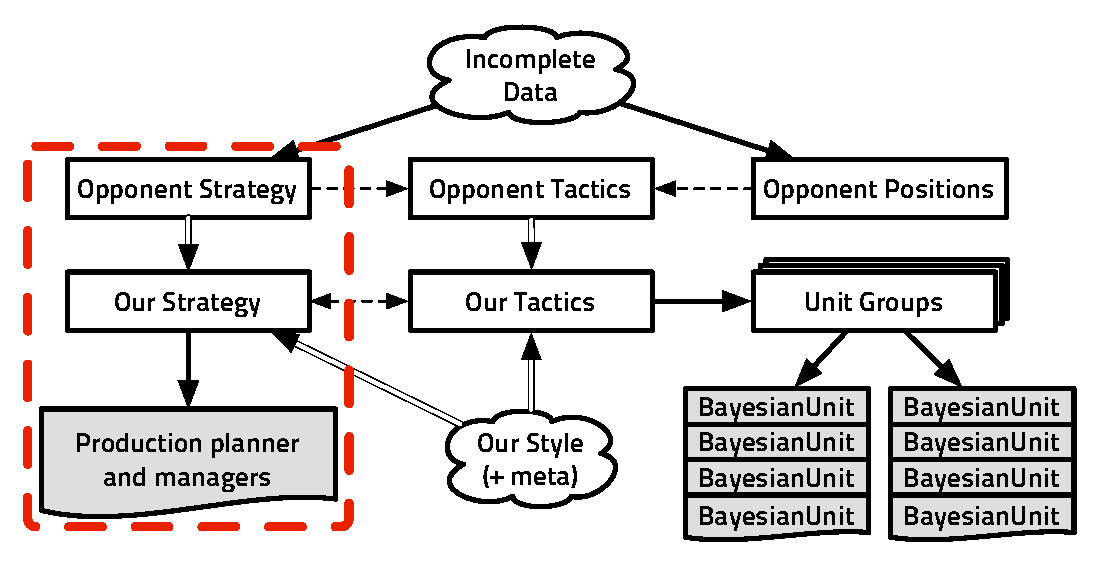
\includegraphics[width=1\columnwidth]{images/starcraft_bbq_concept_STRATEGY.pdf}
\end{center}
\caption{Information-centric view of the architecture of the bot, the part concerning this chapter is in the dotted rectangle}
\label{fig:conceptSTRATEGY}
\end{figure}

\begin{itemize}
\item \underline{Problem:} take the winning strategy in the absolute (knowing everything: complete observations, players intentions, effects of each possible actions).
\item \underline{Problem that we solve:} take the winning strategy (in average) knowing what we saw from the opponent and our model of the game. 
\item \underline{Type:} prediction is a problem of \textit{inference} or \textit{plan recognition} from \textit{incomplete informations}; adaptation given what we know is a problem of \textit{planning under constraints}.
\item \underline{Complexity:} simple StarCraft decision problems are \textsc{np}-hard \citep{GamingComplexity}. We would argue that basic StarCraft strategy with full information (remember that StarCraft is partially observable) is mappable to the Generalized Geography problem\footnote{As the \gloss{techtree} get opened, the choices in this dimension of strategy is being reduced as in Generalized Geography.} and thus is \textsc{pspace}-hard \citep{Lichtenstein78},
Chess \citep{Fraenkel81} and Go (with Japanese ko rules) are \textsc{exptime}-complete \citep{Robson83}. Our solutions are real-time on a laptop. %%% TODO XXX
%\item Results: better resistance to noise, which is fundamental in real setup RTS gameplay (fog of war). Full Bayesian model down to adaptation actions some day?
%\item Conclusion and perspectives: a way to encode and use gameplay/structural knowledge 
\end{itemize}

\section{What is strategy?}
\label{sec:whatisstrategy}
% tech tree, opening, army composition, build tree

%In a RTS, players need to gather resources to build military units and defeat their opponents. To that end, they often have \textit{worker units} (or extraction structures) than can gather resources needed to build \textit{workers}, \textit{buildings}, \textit{military units} and \textit{research upgrades}. Workers are often also builders (as in StarCraft) and are weak in fights compared to military units. Resources may have different uses, for instance in StarCraft: minerals are used for everything, whereas gas is only required for advanced buildings or military units, and technology upgrades. Buildings and research upgrades define technology trees (directed acyclic graphs) and each state of a ``tech tree'' allow for different unit type production abilities and unit spells/abilities. The military can be of different types, any combinations of ranged, casters, contact attack, zone attacks, big, small, slow, fast, invisible, flying... Units can have attacks and defenses that counter each others as in rock-paper-scissors. We consider \textit{strategy} the way to expand the tech tree as well as the army composition, because both require long term planning under uncertainty, and a risk-reward trade-off. 

As it is an abstract concept, what constitutes \textit{strategy} is hard to grasp. The definition that we use for strategy is a combination of aggressiveness and ``where do we put the cursor/pointer/slider between economy, technology and military production?''. It is very much related to where we put our resources:
\begin{itemize}
    \item If we prioritize economy, on a short term basis our army strength (numbers) may suffer, but on the longer term we will be able to produce more, or produce equally and still expand our economy or technology in parallel. Also, keep in mind that resources depletes mineral deposits/gas geysers can be exhausted/drained.
    \item If we prioritize technology, on a short term basis our army strength may suffer, on the longer term it can strive with powerful units or units which are adapted to the enemy's.
    \item If we prioritize military production, on a short term basis our army strength will strive, but we will not be able to adapt our army composition to new unit types nor increase our production throughput.
\end{itemize}
Strategy is a question of balance between these three axis, and of knowing when we can attack and when we should stay in defense. Being aggressive is best when we have a military advantage (in numbers or technology) over the opponent. Advantages are gained by investments in these axis, and capitalizing on them when we max out our returns (comparatively to the opponent's).

The other aspect of strategy is to decide what to do with these resources. This is the part that we studied the most, and the decision-making questions are:
\begin{itemize}
    \item Where do we expand? (We deal with this question by an ad-hoc solution.)
    \item Which tech path do we open? Which tech tree do we want to span in a few minutes? We have to follow a tech tree that enables us to perform the tactics and long term strategy that we want to do, but we also have to adapt to whatever the opponent is doing.
    \item Which unit types, and in which ratios, do we want in our army? We have a choice in units that we can build, they have costs, we have to decide a production plan, knowing the possible evolutions of our tech tree and our possible future production possibilities and capabilities.
\end{itemize}

%The challenges for an AI enabled/empower with strategic reasoning is to be able to assess the strategic situation of the game (both for itself and for the opponent) and to position the two \textit{aggressiveness} and \textit{resources} (eco/tech/army) pointers as best as it can. 
In the following, we studied the estimation of the opponent's strategy in terms of \gloss{techtree} (\gloss{buildtree}), abstracted (labeled) \glos{opening} (early strategy), army composition, and how we should adapt our own strategy to it.

\section{Related work}

%This work was encouraged by the reading of Weber and Mateas' Data Mining Approach to Strategy Prediction \citep{weberStrat} and the fact that they provided their dataset, that we used. They tried and evaluated several machine learning algorithms on replays that were labeled with strategies (openings) with rules.

There are precedent works of Bayesian plan recognition \citep{BMPR}, even in games with \citep{BayesianRecog} using dynamic Bayesian networks to recognize a user's plan in a multi-player dungeon adventure. Commercial RTS games most commonly use \glos{FSM} \citep{FSM_AIGameProgWisdom2003} to encode strategies and their transitions.

There are related works in the domains of opponent modeling \citep{HsiehS08,schadd2007opponent,Kabanza2010}. The main methods used to these ends are case-based reasoning (CBR) and planning or plan recognition \citep{LTW,CBR_Planning,OntanonCBR,HTNPlanning,Ramirez}.

\cite{LTW} used \glos{CBR} to perform dynamic plan retrieval extracted from domain knowledge in Wargus (Warcraft II open source clone). \cite{CBR_Planning} base their real-time case-based planning (CBP) system on a plan dependency graph which is learned from human demonstration in Wargus. In \citep{OntanonCBR,PlanRetrieval}, they use CBR and expert demonstrations on Wargus. %They update their previous CPB approach by using ``situation assessment'' for plan retrieval. 
They improve the speed of CPB by using a decision tree to select relevant features. \cite{HsiehS08} based their work on \citep{LTW} and used StarCraft replays to construct states and building sequences. Strategies are choices of building construction order in their model. 

\cite{schadd2007opponent} describe opponent modeling through hierarchically structured models of the opponent's behavior and they applied their work to the Spring RTS game (Total Annihilation open source clone). \cite{HTNPlanning} use hierarchical task networks (\glos{HTN}) to model strategies in a first person shooter with the goal to use HTN planners. \cite{Kabanza2010} improve the probabilistic hostile agent task tracker (PHATT \citep{PHATT}, a simulated \glos{HMM} for plan recognition) by encoding strategies as HTN. 

\cite{weberStrat} presented ``a data mining approach to strategy prediction'' and performed supervised learning (from buildings features) on labeled StarCraft replays. In this chapter, for openings prediction, we worked with the same dataset as they did, using their openings labels and comparing it to our own labeling method. %\cite{Weber2010qf} applied this automated replay annotation approach to CBP on StarCraft.

\cite{HMMstrat_RTS_AIIDE11} presented their work at the same conference that we presented \citep{SYNNAEVE:StratPred}. They used an HMM which states are extracted from (unsupervised) maximum likelihood on the dataset. The HMM parameters are learned from unit counts (both buildings and military units) every 30 seconds and Viterbi inference is used to predict the most likely next states from partial observations. 

\cite{bjorn2012} augmented the C4.5 decision tree \citep{quinlan1993} and nearest neighbour with generalized examplars \citep{martin1995}, also used by \cite{weberStrat}, with a Bayesian network on the buildings (\glos{buildtree}). Their results confirm ours: the predictive power is strictly better and the resistance to noise far greater than without encoding probabilistic estimations of the \glos{buildtree}.


\section{Perception and interaction}

\subsection{Buildings}
\label{sec:buildings}

From last chapter (section~\ref{sec:techtree}), we recall that the \textit{\glos{techtree}} is a directed acyclic graph which contains the whole technological (buildings and upgrades) development of a player. Also, each unit and building has a \textit{sight range} that provides the player with a view of the map. Parts of the map not in the sight range of the player's units are under \textit{fog of war} and the player ignores what is and happens there. We also recall the notion of \glos{buildorder}: the timings at which the first buildings are constructed. 

In this chapter, we will use \textit{\gloss{buildtree}} as a proxy for estimating some of the strategy. A build tree is a little different than the \glos{techtree}: it is the tech tree without upgrades and researches (only buildings) and augmented of some duplications of buildings. For instance, $\{Pylon\wedge Gateway\}$ and $\{Pylon\wedge Gateway, Gateway2\}$ gives the same tech tree but we consider that they are two different build trees. Indeed, the second Gateway gives some units producing power to the player (it allows for producing two Gateway units at ones). Very early in the game, it also shows investment in production and the strategy is less likely to be focused on quick opening of technology paths/upgrades. 
We have chosen how many different versions of a given building type to put in the build trees (as shown in Table~\ref{tab:labels}), so it is a little more arbitrary than the tech trees. Note that when we know the build tree, we have a very strong conditioning on the tech tree.



\subsection{Openings}
\label{sec:openings}

\newglossaryentry{rush}{name=rush,description={quick aggressive opening}}

In RTS games jargon, an \textit{\glos{opening}} denotes the same thing than in Chess: an early game plan for which the player has to make choices. In Chess because one can not move many pieces at once (each turn), in RTS games because during the development phase, one is economically limited and has to choose between economic and military priorities and can not open several tech paths at once. A \textit{\glos{rush}} is an aggressive attack ``as soon as possible'', the goal is to use an advantage of surprise and/or number of units to weaken a developing opponent. A \textit{push} (also timing push or timing attack) is a solid and constructed attack that aims at striking when the opponent is weaker: either because we reached a wanted army composition and/or because we know the opponent is expanding or ``teching''. The \glos{opening} is also (often) strongly tied to the first military (tactical) moves that will be performed. It corresponds to the 5 (early rushes) to 15 minutes (advanced technology / late push) timespan. 

Players have to find out what opening their opponents are doing to be able to effectively deal with the strategy (army composition) and tactics (military moves: where and when) thrown at them. For that, players scout each other and reason about the incomplete information they can bring together about army and buildings composition. This chapter presents a probabilistic model able to predict the \textit{\glos{opening}} of the enemy that is used in a StarCraft AI competition entry bot. Instead of hard-coding strategies or even considering plans as a whole, we consider the long term evolution of our \glos{techtree} and the evolution of our army composition separately (but steering and constraining each others), as shown in Figure~\ref{fig:conceptSTRATEGY}. With this model, our bot asks ``what units should I produce?'' (assessing the whole situation), being able to revise and adapt its production plans.

Later in the game, as the possibilities of strategies ``diverge'' (as in Chess), there are no longer fixed foundations/terms that we can speak of as for openings. Instead, what is interesting is to know the technologies available to the enemy as well as have a sense of the composition of their army. The players have to adapt to each other's technologies and armies compositions either to be able to defend or to attack. Some units are more cost-efficient than others against particular compositions. Some combinations of units play well with each others (for instance biological units with ``medics'' or a good ratio of strong contact units backed with fragile ranged or artillery units). Finally, some units can be game changing by themselves like cloaking units, detectors, massive area of effects units... 

\subsection{Military units}
\label{sec:militaryunits}
Strategy is not limited to technology state, openings and timings. The player must also take strategic decisions about the army composition. While some special tactics (drops, air raids, invisible attacks) require some specific units, these does not constitute the bulk of the army, at least not after the first stages of the game ($\approx$ 10 minutes).

The different attack types and ``armor'' (size) types of units make it so that pairing units against each others is like a soft rock-paper-scissors (shi-fu-mi). But there is more to army composition than playing rock-paper-scissors with anticipation (units take time to be produced) and partial information: some units combine well with each others. The simplest example of combinations are ranged units and contact units which can be very weak (lots of weaknesses) taken separately, but they form an efficient army when combined. There are also units which empower others through abilities, or units with very strong defensive or offensive abilities with which one unit can change the course of a battle. As stated before, these different units need different parts of the tech tree to be available and they have different resources costs. All things considered, deciding which units to produce is dependent on the opponent's army, the requirements of the planned tactics, the resources and the current (and future) technology available to the player.

\section{Replays labeling}
\label{sec:replayslabeling}

A \glos{replay} contains all the actions of each players during a game. We used a dataset of replays to see when the players build which buildings (see Table~\ref{tab:replay_example} in appendix for an example of the buildings constructions actions). We attributed a label for each player for each game which notes the players \glos{opening}.

\subsection{Dataset}

We used Weber and Mateas \citep{weberStrat} dataset of labeled replays. It is composed of 8806 StarCraft: Broodwar game logs, the details are given in Table~\ref{tab:weberdatasetnumbers}. A \glos{matchup} is a set of the two opponents races: Protoss versus Terran (PvT) is a match-up, Protoss versus Zerg (PvZ) is another one. They are distinguished because strategies distribution are very different across match-ups (see Tables~\ref{tab:weberdatasetnumbers} and \ref{tab:openings_distrib}). Weber and Mateas used logic rules on building sequences to put their labels, concerning only tier 2 strategies (no tier 1 rushes).

\begin{table}[!h]
\begin{center}
\begin{footnotesize}
\begin{tabular}{|l|c|c|c|l|c|c|c|l|c|c|c|}
\hline
opening & PvP & PvT & PvZ & opening & TvP & TvT & TvZ & opening & ZvP & ZvT & ZvZ \\
\hline
FastLegs & 4 & 17 & 108 & Bio & 144 & 41 & 911 & Lurker & 33 & 184 & 1 \\
FastExpand & 119 & 350 & 465 & Unknown & 66 & 33 & 119 & Unknown & 159 & 164 & 212 \\
ReaverDrop & 51 & 135 & 31 & Standard & 226 & 1 & 9 & HydraRush & 48 & 13 & 9 \\
FastObs & 145 & 360 & 9 & SiegeExpand & 255 & 49 & 7 & Standard & 40 & 80 & 1 \\
Unknown & 121 & 87 & 124 & VultureHarass & 134 & 226 & 5 & TwoHatchMuta & 76 & 191 & 738 \\
Carrier & 2 & 8 & 204 & TwoFactory & 218 & 188 & 24 &  HydraMass & 528 & 204 & 14 \\
FastDT & 100 & 182 & 83 & FastDropship & 96 & 90 & 75 & ThreeHatchMuta & 140 & 314 & 35 \\
\hline
total & 542 & 1139 & 1024 & total & 1139 & 628 & 1150 & total & 1024 & 1150 & 1010 \\
\hline
\end{tabular}
\end{footnotesize}
\end{center}
\caption{Weber's dataset with its labels. XvY means the XvY or YvX match-up but the openings numbers are presented for X.}
\label{tab:weberdatasetnumbers}
\end{table}

\subsection{Probabilistic labeling}

Instead of labeling with rules, we used (positive labeling vs rest) clustering of the opening's main features to label the games of each player.

\subsubsection{The pitfall of logical/rule-based labeling}
Openings are closely related to \gloss{buildorder} (BO) but different BO can lead to the same opening and some BO are shared by different openings. Particularly, if we do not take into account the time at which the buildings are constructed, we may have a wrong opening label too often: if an opening consist in having building C as soon as possible, it does not matter if we built B-A-C instead of the standard A-B-C as long as we have built C quickly. That is the kind of case that will be overlooked by logical labeling. For that reason, we tried to label replays with the statistical appearance of key features with a semi-supervised method (see Figure~\ref{fig:replays_labeling}). Indeed, the purpose of our opening prediction model is to help our StarCraft playing bot to deal with rushes and special tactics. This was not the main focus of Weber and Mateas' labels, which follow exactly the build tree. So, we used the key components of openings that we want to be aware of as features for our labeling algorithm as shown in Table~\ref{tab:labels}.

\begin{figure}[h]
\centerline{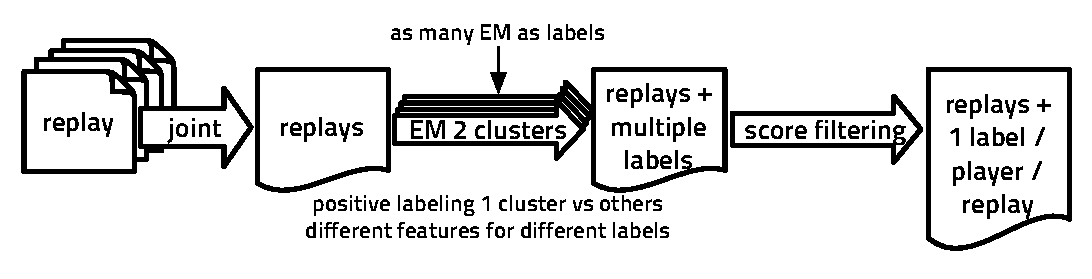
\includegraphics[width=0.80\columnwidth]{images/replays_labeling.pdf}}
\caption{Data centric view of our semi-supervised labeling of replays. 
We put together a replays dataset and pass each game (for each player) through a Gaussian mixtures model (\glos{GMM}) expectation-maximization (\glos{EM}) clustering for each label against the rest. We then filter and keep only the most probable and first to appear \glos{opening} label for each player for each game.}
\label{fig:replays_labeling}
\end{figure}

\subsubsection{Main features of openings}

The selection of the features along with the opening labels is the supervised part of our labeling method. The knowledge of the features and openings comes from expert play and the StarCraft Liquipedia\footnote{\url{http://wiki.teamliquid.net/starcraft/}} (a Wikipedia for StarCraft). They are all presented in Table~\ref{tab:labels}. For instance, if we want to find out which replays correspond to the ``fast Dark Templar'' (DT, Protoss invisible unit) opening, we put the time at which the first Dark Templar is constructed as a feature and perform clustering on replays with it. This is what is needed for our playing bot: to be able to know when he has to fear ``fast DT'' opening and build a detector unit quickly to be able to deal with invisibility.

\begin{table}[h] \caption{Opening/Strategies labels of the replays (Weber's and ours are not always corresponding)}
\begin{footnotesize}
\begin{center}
\begin{tabular}{|c|c|ccc|}
\hline
Race
& Weber's labels
& Our labels
& Features 
& Note (what we fear) \\ \hline
Protoss & FastLegs & speedzeal & Legs, GroundWeapons+1 & quick speed+upgrade attack\\
 & FastDT & fast\_dt & DarkTemplar & invisible units\\
 & FastObs & nony & Goon, Range & quick long ranged attack\\
 & ReaverDrop & reaver\_drop & Reaver, Shuttle & tactical attack zone damages \\
 & Carrier & corsair & Corsair & flying units \\
 & FastExpand & templar & Storm, Templar & powerful zone attack \\
 &  & two\_gates & 2ndGateway, Gateway, & aggressive rush \\
 & & & 1stZealot  & \\
 & Unknown & unknown & (no clear label) & \\ \hline
Terran  & Bio & bio & 3rdBarracks, 2ndBarracks, & aggressive rush\\ 
 & & & Barracks & \\
 & TwoFactory & two\_facto & 2ndFactory & strong push (long range) \\ 
 & VultureHarass & vultures & Mines, Vulture & aggressive harass, invisible\\ 
 & SiegeExpand & fast\_exp\footnote{also sometimes noted ``rax\_fe'', this is not the same as SiegeExpand which requires more technology before expanding.} & Expansion, Barracks & economical advantage \\ 
 & Standard & & & \\ 
 & FastDropship & drop & DropShip & tactical attack \\ 
 & Unknown & unknown & (no clear label) & \\ \hline
Zerg & TwoHatchMuta & fast\_mutas & Mutalisk, Gas & early air raid \\
 & ThreeHatchMuta & mutas & 3rdHatch, Mutalisk & massive air raid \\
 & HydraRush & hydras & Hydra, HydraSpeed, & quick ranged attack\\
 & & & HydraRange  & \\
 & Standard & (speedlings) & (ZerglingSpeed, Zergling) & (removed, quick attacks/mobility) \\
 & HydraMass & & & \\
 & Lurker & lurkers & Lurker & invisible and zone damages \\
 & Unknown & unknown & (no clear label) & \\ \hline
\end{tabular}
\label{tab:labels}
\end{center}
\end{footnotesize}
\end{table}

\begin{table}[h]
\caption{Openings distributions for Terran in all the match-ups. They are the result of the clustering-based labeling with selection of one label per replay and per player. We can see that openings usage is different depending on the \glos{matchup}.}
\begin{center}
\begin{tabular}{|c|cc|cc|cc|}
\hline
&  & vs Protoss &  & vs Terran &  & vs Zerg \\
Opening
& Nb
& \begin{scriptsize}Percentage\end{scriptsize}
& Nb
& \begin{scriptsize}Percentage\end{scriptsize}
& Nb
& \begin{scriptsize}Percentage\end{scriptsize} \\ \hline
%%%two\_gates & 332 & & 252 & & 304 & \\
%%%fast\_dt & 7 & & 87 & & 20 & \\
%%%templar & 3 & & 17 & & 22 & \\
% TvP 1007
% TvT 576
% TvZ 872
bio 	    & 62 	& 6.2 	& 25 	& 4.4   & 197 	& 22.6 \\
fast\_exp 	& 438 	& 43.5 	& 377 	& 65.4  & 392 	& 44.9 \\
two\_facto 	& 240 	& 23.8  & 127 	& 22.0  & 116 	& 13.3 \\
vultures 	& 122 	& 12.1  & 3 	& 0.6   & 3 	& 0.3  \\
drop 	    & 52 	& 5.2   & 10 	& 1.7   & 121 	& 13.9 \\
unknown 	& 93 	& 9.3   & 34 	& 5.9   & 43 	& 5.0 \\ \hline
\end{tabular}
\label{tab:openings_distrib}
\end{center}
\end{table}

%\clearpage

\subsubsection{Clustering}

For the clustering part, we tried k-means and expectation-maximization (\glos{EM}, with Gaussian mixtures) on Gaussian mixtures with shapes and volumes chosen with a Bayesian information criterion (\glos{BIC}). Best BIC models were almost always the most agreeing with expert knowledge (15/17 labels), so we kept this method. We used the R package Mclust \citep{Mclust,Mclust2} to perform full EM clustering. 

\label{GMMEM}
The Gaussian mixture model (\glos{GMM}) is as follows:
\begin{itemize}
    \item Variables:
    \begin{itemize}
        \item $X_{i \in \llbracket 1 \dots n\rrbracket}$ the features for the $i$th replay/game. For instance for the ``fast\_expand'' opening (Barracks and then direct expanding), we used the features ``time of the first expansion'' and ``time of the first Barracks'', as is shown in Figure~\ref{TvZraxFE}, and each data point is an $X_i$.
        \item $Op_{i \in \llbracket1 \dots n\rrbracket}$ the opening of game $i$. Instead of doing one clustering with $k$ possible openings, we did $k$ clusterings of 1 opening vs the rest. So for us $Op_i \in \{opening, rest\}$.
    \end{itemize}
    \item Decomposition ($n$ data points, i.e. $n$ games):
$$\PP(X_{1:n}, Op_{1:n}) = \prod_{i=1}^n \PP(X_i|Op_i)\PP(Op_i)$$
    \item Forms, for the $k$ openings we have:
    \begin{itemize}
        %\item $\PP(X_i|Op_i) = \sum_{j \in \{op,\neg op\}} \mathcal{N}(\mu_j, \sigma_j^2)$ 
        \item $\PP(X_i|Op_i)$ mixture of (two) Gaussian distributions
        \begin{eqnarray*}
            \begin{cases} \PP(X_i|Op_i=op) = \mathcal{N}(\mu_{op}, \sigma_{op}^2)\\
            \PP(X_i|Op_i=\neg op) = \mathcal{N}(\mu_{\neg op}, \sigma_{\neg op}^2) \end{cases} 
        \end{eqnarray*}
        \item $\PP(Op_i) = Bernouilli(p_{op})$: 
        \begin{eqnarray*}
            \begin{cases} \PP(Op_i=op) = p_{op}\\
            \PP(Op_i=\neg op) = 1-p_{op} \end{cases}
        \end{eqnarray*}
    \end{itemize}
    \item Identification (\glos{EM} with maximum likelihood estimate\footnote{Maximum a posteriori (MAP) would maximize the joint.}):\\
    Let $\theta= (\mu_{1:2},\sigma_{1:2})$, initialize $\theta$ randomly, \\
and let $L(\theta;X) = \PP(X|\theta) = \prod_{i=1}^n \sum_{Op_i}\PP(X_i|\theta,Op_i)\PP(Op_i)$
Iterate until convergence (of $\theta$):
    \begin{enumerate}
        \item E-step: $Q(\theta|\theta^{(t)})= \mathrm{E}[\log L(\theta;x,Op)] = \mathrm{E}[\log \prod_{i=1}^n \sum_{Op_i}\PP(x_i|Op_i,\theta)\PP(Op_i)]$
        \item M-step: $\theta^{(t+1)}=\argmax_{\theta} Q(\theta|\theta^{(t)})$
    \end{enumerate}

    \item Question (for the $i$th game):
%$$\PP(Op_{1:n} | X_{1:n}) \propto \PP(X_{1:n}|Op_{1:n})\PP(Op_{1:n})$$
$$\PP(Op_i|X_i=x) = \PP(X_i=x|Op_i)\PP(Op_i)$$
\end{itemize}

%%% Full Bayesian program for (one) GMM trained with EM:
%%% \begin{eqnarray*}
%%% \begin{sideways}\parbox{35mm}{\hspace{-1.3cm}Bayesian program}\end{sideways}
%%% \begin{cases}
%%% \begin{sideways}\parbox{15mm}{\hspace{-0.8cm}Description}\end{sideways}
%%%     \begin{cases}
%%% \begin{sideways}\parbox{35mm}{\hspace{-1.1cm}Specification ($\pi$)}\end{sideways}
%%%         \begin{cases}
%%%             Variables:\\
%%%                 X_{1:n}, Op_{1:n}\\
%%%             Decomposition:\\
%%%                 \PP(X_{1:n}, Op_{1:n}) = \prod_{i=1}^n \PP(X_i|Op_i)\PP(Op_i)\\
%%%             Forms:\\
%%%                 \PP(X_i|Op_i=op) = \mathcal{N}_{\mu_{op},\sigma_{op}^2}\\
%%%                 \PP(Op_i=op) = Bernouilli(p_{op})\\
%%%         \end{cases}\\
%%%         Identification:\ \mathrm{expectation-maximization}\\
%%%     \end{cases}\\
%%%     Question:\\
%%%     \PP(Op_{1:n} | X_{1:n}) \propto \PP(X_{1:n}|Op_{1:n})\PP(Op_{1:n})\\
%%% \end{cases}
%%% \end{eqnarray*}

\noindent{The $\sigma_j$ matrices can define Gaussian distribution of any combinations between:}
\begin{itemize}
    \item volume (of the normal distributions of each mixtures at a given $\sigma$ value): equal or variable,
    \item shape (of the multidimensional normal distributions of each mixtures): equal or variable, 
    \item orientation: spherical (i.e. no orientation), coordinate axes, equal (any orientation although the same for all mixtures components) or variable (any orientation for any component).
\end{itemize}
A $\sigma$ with variable volume, variable shape and variable orientation is also called a full covariance matrix. We chose the combinations with the best (i.e. smallest) \glos{BIC} score. For a given model with $n$ data points, $m$ parameters and $L$ the maximum likelihood, $BIC= -2 \ln(L) + m \ln(n)$. 

\begin{figure}[hp]
\centerline{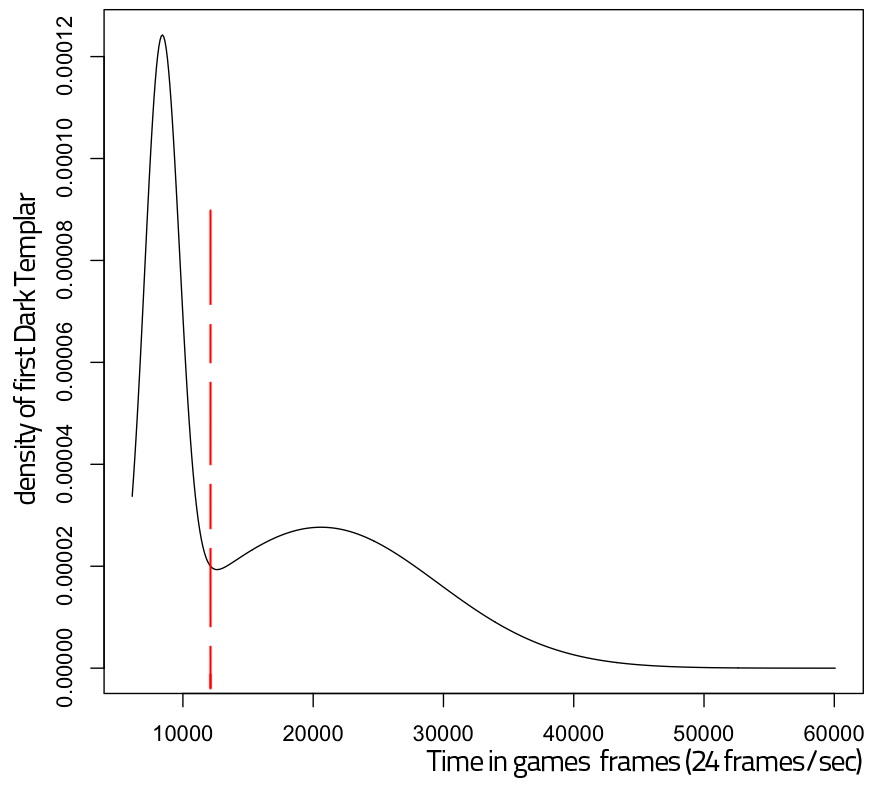
\includegraphics[width=0.56\columnwidth]{images/PvTfastDT.png}}
\caption{Protoss vs Terran distribution of first appearance of Dark Templars (Protoss invisible unit) for the ``fast\_dt'' label (left mode) vs the rest (right mode).}
\label{PvTfastDT}
\end{figure}

\begin{figure}[h]
\centerline{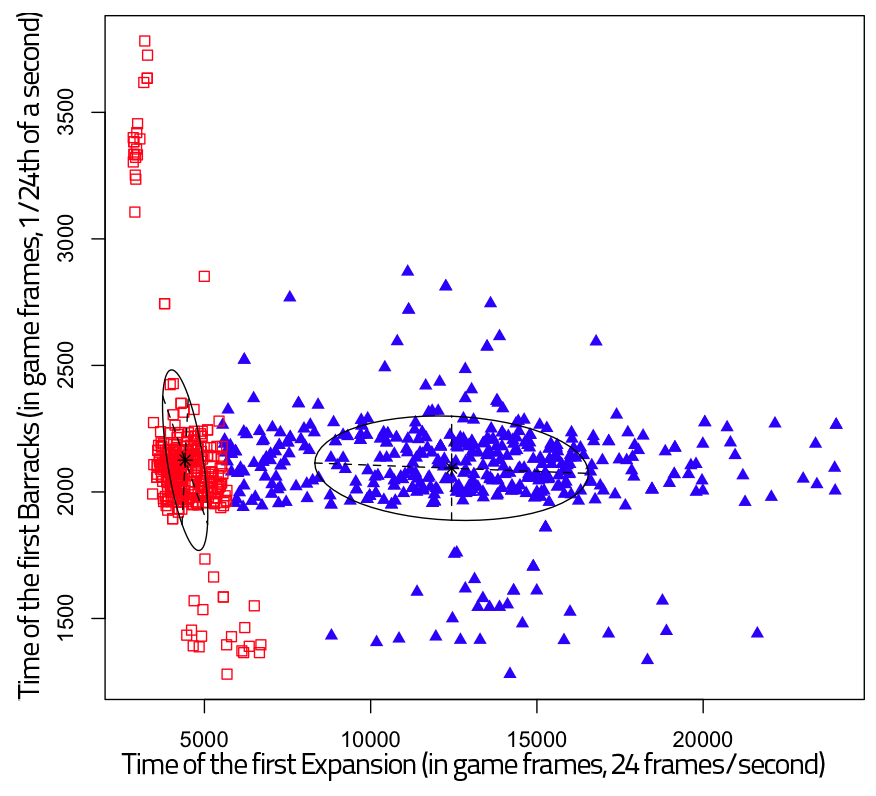
\includegraphics[width=0.72\columnwidth]{images/TvZraxFE.png}}
\caption{Terran vs Zerg Barracks and first Expansion timings (Terran). The bottom left cluster (square data points) is the one labeled as \textit{fast\_exp}. Variable volume, variable shape, variable orientation covariance matrices.}
\label{TvZraxFE}
\end{figure}

\begin{figure}[h]
\centerline{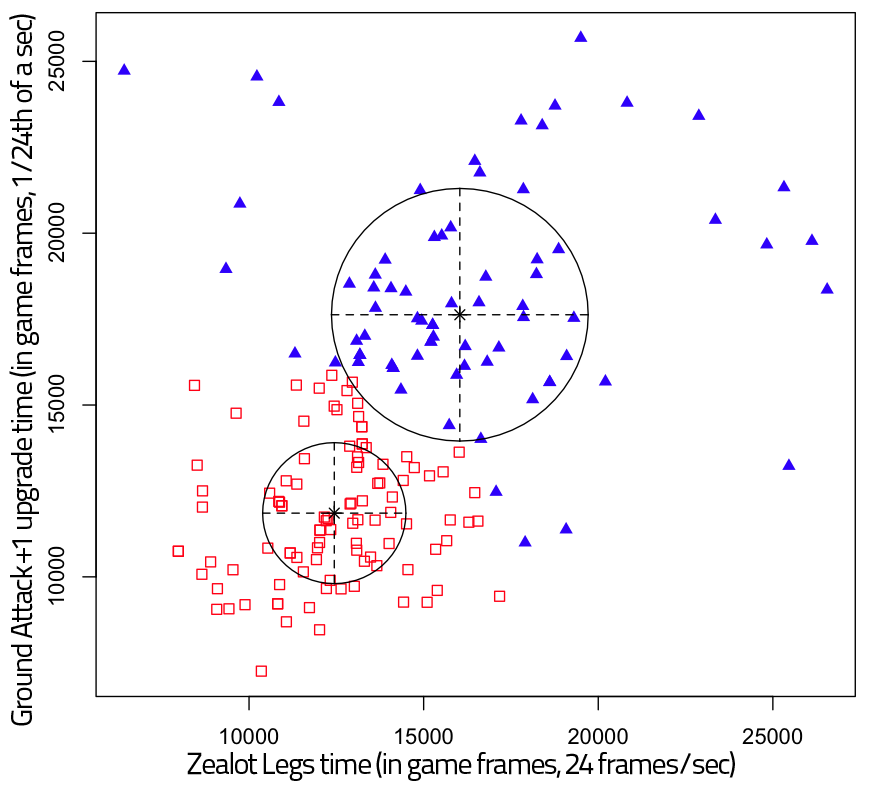
\includegraphics[width=0.66\columnwidth]{images/PvPspeedzeal.png}}
\caption{Protoss vs Protoss Ground Attack +1 and Zealot Legs upgrades timings. The bottom left cluster (square data points) is the one labeled as \textit{speedzeal}. Variable volume, equal shape, spherical covariance matrices.}
\label{PvPspeedzeal}
\end{figure}

\begin{figure}[h]
\centerline{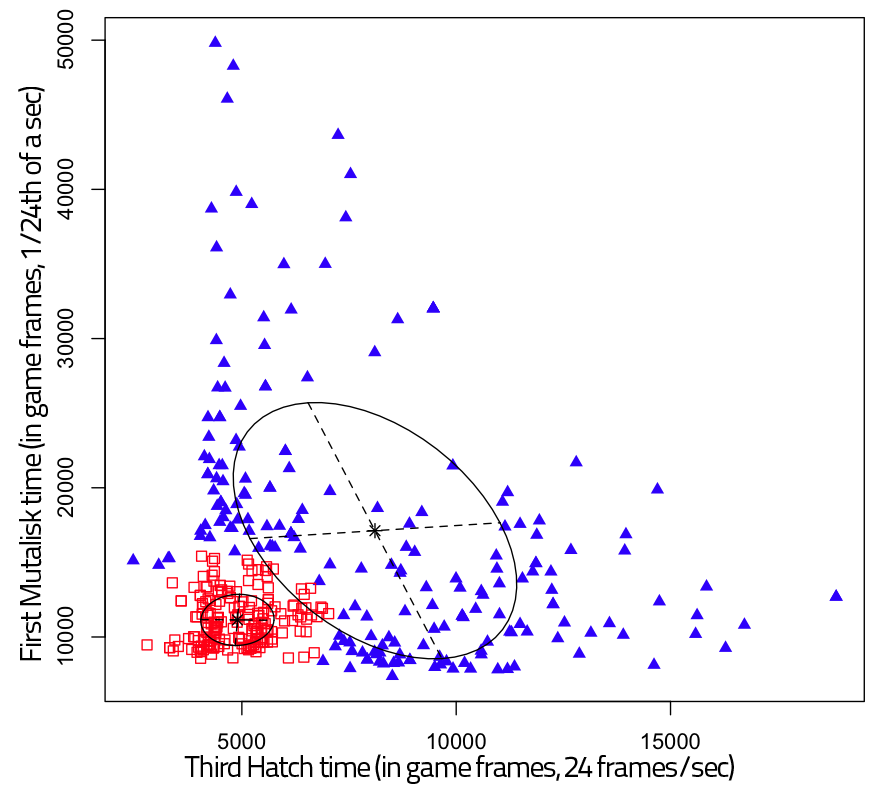
\includegraphics[width=0.66\columnwidth]{images/ZvPmutas.png}}
\caption{Zerg vs Protoss time of the third Hatch and first appearance of Mutalisks. The bottom left cluster (square data points) is the one labeled as \textit{mutas}. Variable volume, variable shape, variable orientation covariance matrices.}
\label{ZvPmutas}
\end{figure}



\subsubsection{Labeling, score filtering}
The whole process of labeling replays (games) is shown in Figure~\ref{fig:replays_labeling}.
We produce ``2 bins clustering'' for each set of features (corresponding to each opening), and label the replays belonging to the cluster with the lower norm of features' appearances (that is exactly the purpose of our features). Figures~\ref{PvPspeedzeal}, \ref{TvZraxFE}
and \ref{ZvPmutas} show the clusters out of EM with the features of the corresponding openings. We thought of clustering because there are two cases in which you build a specific military unit or research a specific upgrade: either it is part of your opening, or it is part of your longer term game plan or even in reaction to the opponent. So the distribution over the time at which a feature appears is bimodal, with one (sharp) mode corresponding to ``opening with it'' and the other for the rest of the games, as can be seen in Figure~\ref{PvTfastDT}.

%Finally, some replays are labeled two or three times with different labels (due to the different time of effect of different openings), so we apply a score filtering to transform multiple label replays into unique label ones (see Figure~\ref{replays_labeling}). 
Due to the different time of effect of different openings, some replays are labeled two or three times with different labels. So, finally, we apply a score filtering to transform multiple label replays into unique label ones (see Figure~\ref{fig:replays_labeling}). 
For that we choose the openings labels that were happening the earliest (as they are a closer threat to the bot in a game setup) if and only if they were also the most probable or at 10\% of probability of the most probable label (to exclude transition boundaries of clusters) for this replay. We find the earliest by comparing the norms of the clusters means in competition. All replays without a label or with multiple labels (\textit{i.e.} which did not had a unique solution in filtering) after the filtering were labeled as \textit{unknown}. An example of what is the final distribution amongst replays' openings labels is given for the three Terran \gloss{matchup} in Table~\ref{tab:openings_distrib}. We then used this labeled dataset as well as Weber and Mateas' labels in the testing of our Bayesian model for opening prediction.

\clearpage

\section{Build tree prediction}
\label{sec:strategyprediction}
The work described in the next two sections can be classified as probabilistic plan recognition. Strictly speaking, we present model-based machine learning used for prediction of plans, while our model is not limited to prediction. We performed two levels of plan recognition, both are learned from the replays: tech tree prediction (unsupervised, it does not need openings labeling, this section) and opening prediction (semi-supervised or supervised depending on the labeling method, next section).

\label{sec:techtreepred}

\subsection{Bayesian model}
\subsubsection{Variables}
\begin{itemize}
\item BuildTree: $BT \in \{\emptyset, \{building_1\}, \{building_2\}, \{building_1\wedge building_2\}, \dots\}$: all the possible building trees for the given race. For instance $\{pylon, gate\}$ and $\{pylon, gate, core\}$ are two different $BuildTrees$.
\item Observations: $O_{i \in \llbracket 1\dots N \rrbracket} \in \{0, 1\}$, $O_k$ is $1/true$ if we have seen (observed) the $k$th building (it can have been destroyed, it will stay ``seen''). Otherwise, it is $0/false$.
\item $\lambda \in \{0, 1\}$: coherence variable (restraining $BuildTree$ to possible values with regard to $O_{1:N}$)
\item Time: $T \in \llbracket 1\dots P \rrbracket$, time in the game (1 second resolution).
\end{itemize}

At first, we generated all the possible (according to the game rules) \gloss{buildtree} (BT values) of StarCraft, and there are between $\approx 500$ and $1600$ depending on the race without even counting buildings duplicates! We observed that a lot of possible build trees are too absurd to be performed in a competitive match and were never seen during the learning. So, we restricted $BT$ to have its value in all the build trees encountered in our replays dataset and we added multiple instances of the basic unit producing buildings (gateway, barracks), expansions and supply buildings (depot, pylon, ``overlord'' as a building), as shown in Table~\ref{tab:labels}. 
%%%There are 292 build trees for Terran, 176 for Protoss and 113 for Zerg ($\approx 3000$ replays/race), all learned from the (unlabeled) replays.
This way, there are 810 build trees for Terran, 346 for Protoss and 261 for Zerg (learned from $\approx 3000$ games for each race, see Table~\ref{tab:weberdatasetnumbers}). In a new game, if we encounter a build tree that we never saw, we are in a unknown state. Anyway we would not have seen enough data (any at all) during the learning to conclude anything. We could look at the proximity of the build tree to other known build trees, see section~\ref{sec:buildtreemetrics} and the Discussion (\ref{sec:buildtreeimprovements}).

\subsubsection{Decomposition}
The joint distribution of our model is the following:
%%% \begin{eqnarray*}
%%% & & \PP(T, BT, O_1 \dots O_N, \lambda) \\ 
%%% & = & \PP(T | BT)\PP(BT)\\
%%% & & \times \PP(\lambda | BT, O_{1:N})\prod_{i=1}^{N}\PP(O_{i}) 
%%% \end{eqnarray*}
\begin{equation}
\PP(T, BT, O_1 \dots O_N, \lambda) = \PP(T | BT)\PP(BT) \PP(\lambda | BT, O_{1:N})\prod_{i=1}^{N}\PP(O_{i}) 
\end{equation}
This can also be see as a plate diagram in Figure~\ref{fig:buildtreeplate}.

\begin{figure}[h]
\begin{center}
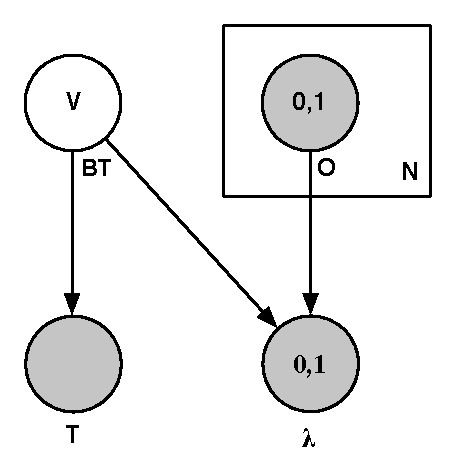
\includegraphics[width=0.35\columnwidth]{images/BuildTreePrediction_plate.pdf}
\end{center}
\caption{Graphical model (plate notation) of the build tree Bayesian model, gray variables are known.}
\label{fig:buildtreeplate}
\end{figure}

\subsubsection{Forms}
\begin{itemize}
\item $\PP(BT)$ is the prior distribution on the build trees. As we do not want to include any bias, we set it to the uniform distribution.

\item $\PP(O_{1:N})$ is unspecified, we put the uniform distribution (we could use a prior over the most frequent observations).

\item $\PP(\lambda | BT, O_{1:N})$ is a functional Dirac that restricts $BT$ values to the ones than can co-exist with the observations:
%%% \begin{eqnarray*}
%%% & & \PP(\lambda = 1 | bt, o_{1:N}) \\
%%% & = & 1\ \mathrm{if\ } bt \ \mathrm{can\ exist\ with\ } o_{1:N} \\
%%% & = & 0\ \mathrm{else}
%%% \end{eqnarray*}
\begin{eqnarray*}
\begin{cases}
\PP(\lambda = 1 | bt, o_{1:N}) = 1\ \mathrm{if\ } bt \ \mathrm{can\ exist\ with\ } o_{1:N} \\
\PP(\lambda = 1 | bt, o_{1:N}) = 0\ \mathrm{else}
\end{cases}
\end{eqnarray*}
A build tree value ($bt$) is compatible with the observations if it covers them fully. For instance, $BT=\{pylon, gate, core\}$ is compatible with $o_{core} = 1$ but it is not compatible with $o_{forge} = 1$. In other words, $buildTree$ is incompatible with $o_{1:N}$ \textit{iff} $\{o_{1:N} \backslash \{o_{1:N} \wedge buildTree\}\} \neq \emptyset$.

\item $\PP(T|BT=bt) = \mathcal{N}(\mu_{bt},\sigma_{bt}^2)$: $\PP(T | BT)$ are discrete normal distributions (``bell shapes''). 
There is one bell shape over $T$ per $bt$. The parameters of these discrete Gaussian distributions are learned from the replays.
\end{itemize}

\subsubsection{Identification (learning)}
As we have full observations in the training phase, learning is just counting and averaging. The learning of the $\PP(T | BT)$ bell shapes parameters takes into account the uncertainty of the $bt$ for which we have few observations: the normal distribution $\PP(T|bt)$ begins with a high $\sigma_{bt}^2$, and \textbf{not} a strong peak at $\mu_{bt}$ on the seen $T$ value and $sigma=0$. This accounts for the fact that the first(s) observation(s) may be outlier(s). This learning process is independent on the order of the stream of examples, seeing point A and then B or B and then A in the learning phase produces the same result. 

\subsubsection{Questions}
%%%\begin{eqnarray*}
%%%P(Op|T=t, O_{1:N}=o_{1:N}, \lambda = 1) \\
%%%\propto \frac{1} {P(o_{1:N}).P(\lambda).P(t)} \\
%%%\sum_{BuildTree} P(Op).P(BuildTree|Op).P(o_{1:N})\\
%%%.P(\lambda|BuildTree,o_{1:N}).P(t|BuildTree,Op)
%%%\end{eqnarray*}
The question that we will ask in all the benchmarks is:
\begin{equation}
\PP(BT|T=t, O_{1:N}=o_{1:N}, \lambda = 1)  \propto \PP(t|BT)\PP(BT) \PP(\lambda | BT, o_{1:N})\prod_{i=1}^N\PP(o_{i})
\end{equation}
An example of the evolution of this question with new observations is depicted in Figure~\ref{fig:ttinf}, in which we can see that build trees (possibly closely related) succeed each others (normal) until convergence.
%Note that if we see $\PP(BT, T)$ as a plan, asking $\PP(BT | T)$ for ourselves boils down to use our ``plan recognition'' mode as a planning algorithm. %, which could provide good approximations of the optimal goal set \cite{Ramirez}, or build orders. %%%This gives us a distribution on the build orders that we can follow.

\subsubsection{Bayesian program}
The full Bayesian program is:
\begin{eqnarray*}
\begin{sideways}\parbox{20mm}{\hspace{-1.3cm}Bayesian program}\end{sideways}
\begin{cases}
\begin{sideways}\parbox{15mm}{\hspace{-0.8cm}Description}\end{sideways}
    \begin{cases}
\begin{sideways}\parbox{18mm}{\hspace{-1.1cm}Specification ($\pi$)}\end{sideways}
        \begin{cases}
        Variables\\
    T, BT, O_1 \dots O_N, \lambda \\ 
        Decomposition\\
            \PP(T, BT, O_1 \dots O_N, \lambda) = JD \\ 
        =   \PP(\lambda | BT, O_{\llbracket 1 \dots N\rrbracket}) \PP(T | BT) \prod_{i=1}^N\PP(O_{i})\PP(BT) \\
        Forms\\
            \PP(\lambda | BT, O_{\llbracket 1 \dots N\rrbracket}) = functional\ Dirac\ \mathrm{(coherence)}\\ 
            \PP(T|BT=bt) = discrete\ \mathcal{N}(\mu_{bt},\sigma_{bt}^2)\\
        \end{cases}\\
    Identification\\
            \PP(BT=bt | Op^t=op) = \frac{1 + \mathrm{count}(bt,op)}{\abs{BT} + \mathrm{count}(op)}\\
            (\mu_{bt},\sigma_{bt}) = \argmax_{\mu,\sigma}\PP(T|BT=bt; \mu,\sigma^2)\\
%%% \mathrm{maximum\ likelihood\ }\{(\mu,\sigma^2)\}\\
    \end{cases}\\
Question \\
\PP(BT|T=t, O_{1:N}=o_{1:N}, \lambda = 1)  \propto \PP(t|BT)\PP(BT) \PP(\lambda | BT, o_{1:N})\prod_{i=1}^N\PP(o_{i})
\end{cases}
\end{eqnarray*}

\begin{figure}
\centerline{\includegraphics[width=0.72\columnwidth]{images/techtree_inference_color3.png}}
\caption{Evolution of $\PP(BT|observations,time,\lambda=1)$ in time (seen/observed buildings on the x-axis). Only $BT$ with a probability $> 0.01$ are shown. The numbers in the legend correspond to build trees identifier numbers. The interpolation was obtained by fitting a second order polynomial.}
\label{fig:ttinf}
\end{figure}


\subsection{Results}
All the results presented in this section represents the nine match-ups (races combinations) in 1 versus 1 (duel) of StarCraft. We worked with a dataset of 8806 replays ($\approx$ 1000 per match-up) of skilled human players (see \ref{tab:weberdatasetnumbers}) and we performed cross-validation with 9/10th of the dataset used for learning and the remaining 1/10th of the dataset used for evaluation. Performance wise, the learning part (with $\approx$ 1000 replays) takes around $0.1$ second on a 2.8 Ghz Core 2 Duo CPU (and it is serializable). Each inference (question) step takes around $0.01$ second. The memory footprint is around 3Mb on a 64 bits machine.

\subsubsection{Metrics}
\label{sec:buildtreemetrics}
$k$ is the numbers of buildings ahead that we can accurately predict the build tree of the opponent at a fixed $d$. $d$ values are distances between the predicted build tree(s) and the reality (at fixed $k$).

The \textbf{robustness to noise} is measured by the distance $d$ to the real build tree with increasing levels of noise, for $k=0$.

The \textbf{predictive power} of our model is measured by the $k>0$ next buildings for which we have ``good enough'' prediction of future build trees in:
$$\PP(BT^{t+k} | T=t, O_{1:N}=o_{1:N}, \lambda = 1)$$

``Good enough'' is measured by a \textbf{distance} $d$ to the actual build tree of the opponent that we tolerate. We used a set distance: $d(bt_1, bt_2) = \mathrm{card}(bt_1 \Delta bt_2) = \mathrm{card}((bt_1\bigcup bt_2) \backslash (bt_1\bigcap bt_2))$. One less or more building in the prediction is at a distance of $1$ from the actual build tree. The same set of buildings except for one replacement is at a distance of $2$ (that would be $1$ is we used tree edit distance with substitution). 
\begin{itemize}
    \item We call $d(best,real)=$``best'' the distance between the most probable build tree and the one that actually happened.
    \item We call $d(bt,real)*\PP(bt)$=``mean'' the marginalized distance between what was inferred balanced (variable $bt$) by the probability of inferences ($\PP(bt)$). 
\end{itemize} 
Note that this distance is always over the \textbf{complete} build tree, and not only the newly inferred buildings. This distance metric was counted only after the fourth (4th) building so that the first buildings would not penalize the prediction metric (the first building can not be predicted 4 buildings in advance). 

For information, the first 4 buildings for a Terran player are more often amongst his first supply depot, barracks, refinery (gas), and factory or expansion or second barracks. For Zerg, the first 4 buildings are is first overlord, zergling pool, extractor (gas), and expansion or lair tech. For Protoss, it can be first pylon, gateway, assimilator (gas), cybernectics core, and sometimes robotics center, or forge or expansion.


Table~\ref{tab:buildtreeresults} shows the \textbf{full results}, the first line has to be interpreted as ``without noise, the average of the following measures are'' (columns):
\begin{itemize}
    \item $d$ for $k=0$:
        \begin{itemize}
            \item $d(best,real) = 0.535$, it means that the average distance from the most probable (``best'') build tree to the real one is 0.535 building.
            \item $d(bt,real)*\PP(bt) = 0.870$, it means that the average distance from each value $bt$ of the distribution on $BT$, weighted by its own probability ($\PP(bt)$), to the real one is 0.87 building.
        \end{itemize}
    \item $k$ for $d=1$:
        \begin{itemize}
            \item best $k=1.193$, it means that the average number of buildings ahead (of their construction) that the model predicts at a fixed maximum error of 1 ($d=1$) for the most probable build tree (``best'') is 1.193 buildings.
            \item ``mean'' $k=3.991$, it means that the average number of buildings ahead (of their construction) that the model predicts at a fixed maximum error 1 ($d=1$), summed for $bt$ in $BT$ value and weighted by $\PP(bt)$ is 3.991\footnote{This shows that when the most probable build tree is mistaken, there is 1) not much confidence in it (otherwise we would have $\PP(bt_{best}) \approx 1.0$ and the ``mean'' $k$ for fixed $d$ values would equal the ``best'' one). 2) much information in the distribution on $BT$, in the subsequent $\PP(bt_{\neg best})$ values.}
        \end{itemize}
    \item idem that the bullet above but $k$ for $d=2$ and $d=3$.
\end{itemize}
The second line (``min'') is the minimum across the different \gloss{matchup} (as they are detailed for $noise=10\%$), the third (``max'') is for the maximum across match-ups, both still at zero noise. Subsequent sets of lines are for increasing values of noise (i.e. missing observations).

\subsubsection{Predictive power}
To test the predictive power of our model, we are interested at looking at how big $k$ is (how much ``time'' before we can predict a build tree) at fixed values of $d$. We used $d=1,2,3$: with $d=1$ we have a very strong sense of what the opponent is doing or will be doing, with $d=3$, we may miss one key building or the opponent may have switched of tech path. 

We can see in Table~\ref{tab:buildtreeresults} that with $d=1$ and without noise (first line), our model predicts in average more than one building in advance ($k>1$) what the opponent will build next if we use only its best prediction. If we marginalize over $BT$ (sum on $BT$ weighted by $\PP(bt)$), we can almost predict \textbf{four} buildings in advance. Of course, if we accept more error, the predictive power (number of buildings ahead that our model is capable to predict) increases, up to $6.122$ (in average) for $d=3$ without noise.


\begin{table*}[h]
\caption{Summarization of the main results/metrics, one full results set for 10\% noise}
\begin{center}
\begin{footnotesize}
\begin{tabular}{|c|c|cc|cc|cc|cc|}
\hline
  & measure & \multicolumn{2}{|c|}{$d$ for $k=0$} & \multicolumn{2}{|c|}{$k$ for $d=1$} & \multicolumn{2}{|c|}{$k$ for $d=2$} & \multicolumn{2}{|c|}{$k$ for $d=3$} \\
 noise & & \begin{scriptsize}$d(best,real)$\end{scriptsize} 
& \begin{scriptsize}$d(bt,real)*\PP(bt)$\end{scriptsize}
& \begin{scriptsize}best\end{scriptsize}
& \begin{scriptsize}``mean''\end{scriptsize}
& \begin{scriptsize}best\end{scriptsize}
& \begin{scriptsize}``mean''\end{scriptsize}
& \begin{scriptsize}best\end{scriptsize}
&  \begin{scriptsize}``mean''\end{scriptsize} \\
\hline
\multirow{3}{3mm}{\begin{sideways}\parbox{3mm}{0\%\ \ }\end{sideways}}
& average & 0.535 & 0.870 & 1.193 & 3.991 & 2.760 & 5.249 & 3.642 & 6.122\\
& min & 0.313 & 0.574 & 0.861 & 2.8 & 2.239 & 3.97 & 3.13 & 4.88\\
& max & 1.051 & 1.296 & 2.176 & 5.334 & 3.681 & 6.683 & 4.496 & 7.334\\
\hline
\multirow{3}{3mm}{\begin{sideways}\parbox{3mm}{10\%\ \ }\end{sideways}}
 & PvP & 0.397 & 0.646 & 1.061 & 2.795 & 2.204 & 3.877 & 2.897 & 4.693\\
 & PvT & 0.341 & 0.654 & 0.991 & 2.911 & 2.017 & 4.053 & 2.929 & 5.079\\
 & PvZ & 0.516 & 0.910 & 0.882 & 3.361 & 2.276 & 4.489 & 3.053 & 5.308\\
 & TvP & 0.608 & 0.978 & 0.797 & 4.202 & 2.212 & 5.171 & 3.060 & 5.959\\
 & TvT & 1.043 & 1.310 & 0.983 & 4.75 & 3.45 & 5.85 & 3.833 & 6.45\\
 & TvZ & 0.890 & 1.250 & 1.882 & 4.815 & 3.327 & 5.873 & 4.134 & 6.546\\
 & ZvP & 0.521 & 0.933 & 0.89 & 3.82 & 2.48 & 4.93 & 3.16 & 5.54\\
 & ZvT & 0.486 & 0.834 & 0.765 & 3.156 & 2.260 & 4.373 & 3.139 & 5.173\\
 & ZvZ & 0.399 & 0.694 & 0.9 & 2.52 & 2.12 & 3.53 & 2.71 & 4.38\\
& average & 0.578 & 0.912 & 1.017 & 3.592 & 2.483 & 4.683 & 3.213 & 5.459\\
& min & 0.341 & 0.646 & 0.765 & 2.52 & 2.017 & 3.53 & 2.71 & 4.38\\
& max & 1.043 & 1.310 & 1.882 & 4.815 & 3.45 & 5.873 & 4.134 & 6.546\\
\hline
\multirow{3}{3mm}{\begin{sideways}\parbox{3mm}{20\%\ \ }\end{sideways}}
& average & 0.610 & 0.949 & 0.900 & 3.263 & 2.256 & 4.213 & 2.866 & 4.873\\
& min & 0.381 & 0.683 & 0.686 & 2.3 & 1.858 & 3.25 & 2.44 & 3.91\\
& max & 1.062 & 1.330 & 1.697 & 4.394 & 3.133 & 5.336 & 3.697 & 5.899\\
\hline
\multirow{3}{3mm}{\begin{sideways}\parbox{3mm}{30\%\ \ }\end{sideways}}
& average & 0.670 & 1.003 & 0.747 & 2.902 & 2.055 & 3.801 & 2.534 & 4.375\\
& min & 0.431 & 0.749 & 0.555 & 2.03 & 1.7 & 3 & 2.22 & 3.58\\
& max & 1.131 & 1.392 & 1.394 & 3.933 & 2.638 & 4.722 & 3.176 & 5.268\\
\hline
\multirow{3}{3mm}{\begin{sideways}\parbox{3mm}{40\%\ \ }\end{sideways}}
& aerage & 0.740 & 1.068 & 0.611 & 2.529 & 1.883 & 3.357 & 2.20 & 3.827\\
& min & 0.488 & 0.820 & 0.44 & 1.65 & 1.535 & 2.61 & 1.94 & 3.09\\
& max & 1.257 & 1.497 & 1.201 & 3.5 & 2.516 & 4.226 & 2.773 & 4.672\\
\hline
\multirow{3}{3mm}{\begin{sideways}\parbox{3mm}{50\%\ \ }\end{sideways}}
& average & 0.816 & 1.145 & 0.493 & 2.078 & 1.696 & 2.860 & 1.972 & 3.242\\
& min & 0.534 & 0.864 & 0.363 & 1.33 & 1.444 & 2.24 & 1.653 & 2.61\\
& max & 1.354 & 1.581 & 1 & 2.890 & 2.4 & 3.613 & 2.516 & 3.941\\
\hline
\multirow{3}{3mm}{\begin{sideways}\parbox{3mm}{60\%\ \ }\end{sideways}}
& average & 0.925 & 1.232 & 0.400 & 1.738 & 1.531 & 2.449 & 1.724 & 2.732\\
& min & 0.586 & 0.918 & 0.22 & 1.08 & 1.262 & 1.98 & 1.448 & 2.22\\
& max & 1.414 & 1.707 & 0.840 & 2.483 & 2 & 3.100 & 2.083 & 3.327\\
\hline
\multirow{3}{3mm}{\begin{sideways}\parbox{3mm}{70\%\ \ }\end{sideways}}
& average & 1.038 & 1.314 & 0.277 & 1.291 & 1.342 & 2.039 & 1.470 & 2.270\\
& min & 0.633 & 0.994 & 0.16 & 0.79 & 1.101 & 1.653 & 1.244 & 1.83\\
& max & 1.683 & 1.871 & 0.537 & 1.85 & 1.7 & 2.512 & 1.85 & 2.714\\
\hline
\multirow{3}{3mm}{\begin{sideways}\parbox{3mm}{80\%\ \ }\end{sideways}}
& average & 1.134 & 1.367 & 0.156 & 0.890 & 1.144 & 1.689 & 1.283 & 1.831\\
& min & 0.665 & 1.027 & 0.06 & 0.56 & 0.929 & 1.408 & 1.106 & 1.66\\
& max & 1.876 & 1.999 & 0.333 & 1.216 & 1.4 & 2.033 & 1.5 & 2.176\\
\hline
\end{tabular}
\label{tab:buildtreeresults}
\end{footnotesize}
\end{center}
\end{table*}


\subsubsection{Robustness to missing informations (``noise'')}
The robustness of our algorithm is measured by the quality of the predictions of the build trees for $k=0$ (reconstruction, estimation) or $k>0$ (prediction) with missing observations in:
$$ \PP(BT^{t+k} | T=t, O_{1:N}=partial(o_{1:N}), \lambda = 1)$$

The ``reconstructive'' power (infer what has not been seen) ensues from the learning of our parameters from real data: even in the set of build trees that are possible, with regard to the game rules, only a few will be probable at a given time and/or with some key structures. %Abiding by probability theory gives us consistency with regard to concurrent build tree.
The fact that we have a distribution on $BT$ allows us to compare different values $bt$ of $BT$ on the same scale and to use $\PP(BT)$ (``soft evidence'') as an \textbf{input} in other models. 
This ``reconstructive'' power of our model is shown in Table~\ref{tab:buildtreeresults} with $d$ (distance to actual building tree) for increasing noise at fixed $k=0$. 

Figure~\ref{fig:buildtreenoise} displays first (on top) the evolution of the error rate in reconstruction (distance to actual building) with increasing random noise (from 0\% to 80\%, no missing observations to 8 missing observations over 10). We consider that having an average distance to the actual build tree a little over $1$ for 80\% missing observations is a success. This means that our reconstruction of the enemy build tree with a few rightly timed observations is very accurate. We should ponder that this average ``missed'' (unpredicted or wrongly predicted) building can be very important (for instance if it unlocks game changing technology). We think that this robustness to noise is due to $\PP(T|BT)$ being precise with the amount of data that we used, and the build tree structure. 

Secondly, Figure~\ref{fig:buildtreenoise} displays (at the bottom) the evolution of the predictive power (number of buildings ahead from the build tree that it can predict) with the same increase of noise. Predicting 2 building ahead with $d=1$ (1 building of tolerance) gives that we predict right (for sure) at least one building, at that is realized up to almost 50\% of noise. In this case, this ``one building ahead'' right prediction (with only 50\% of the information) can give us enough time to adapt our strategy (against a game changing technology).

\begin{figure}[htp]
\begin{center}
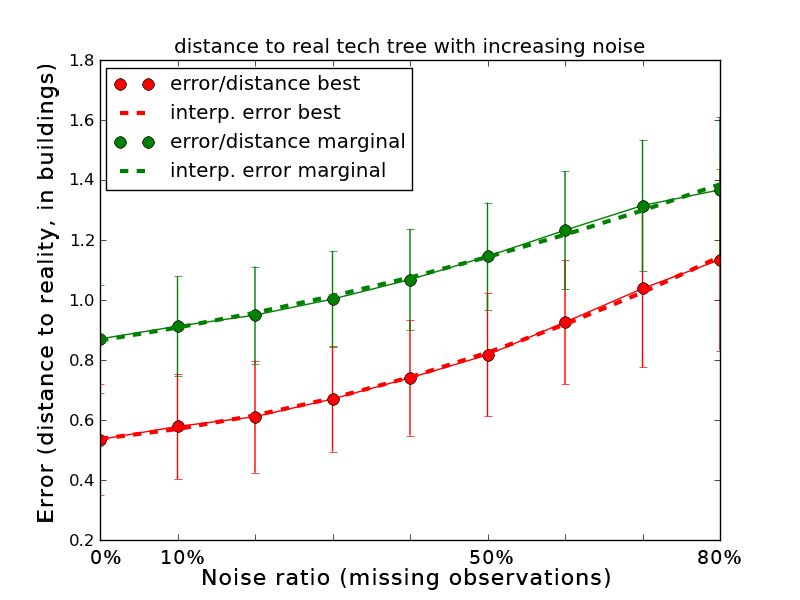
\includegraphics[width=0.7\columnwidth]{images/error_noise2.png}\\
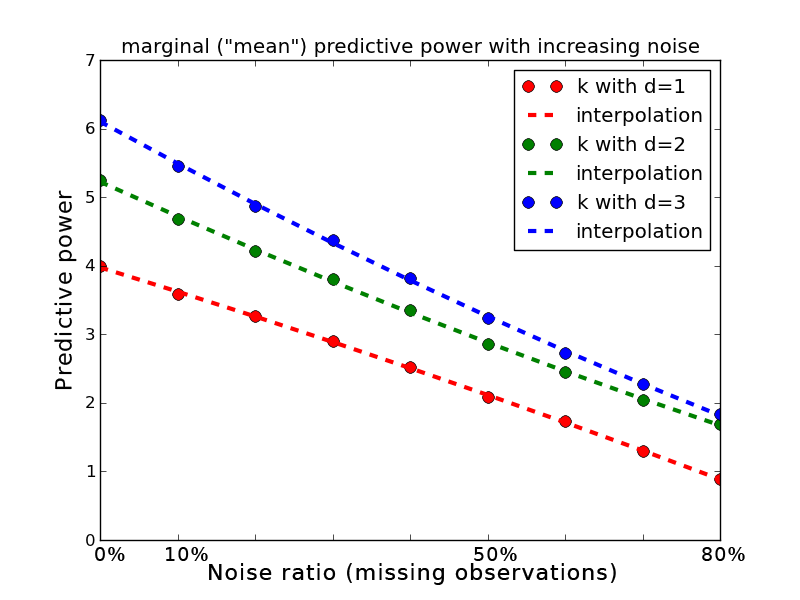
\includegraphics[width=0.7\columnwidth]{images/predictive_power_noise2.png}
\end{center}
\caption{Evolution of our metrics with increasing noise, from 0 to 80\%. The top graphic shows the increase in distance between the predicted build tree, both most probable (``best'') and marginal (``mean'') and the actual one. The bottom graphic shows the decrease in predictive power: numbers of buildings ahead ($k$) for which our model predict a build tree closer than a fixed distance/error ($d$).}
\label{fig:buildtreenoise}
\end{figure}

\subsection{Possible improvements}
%\subsubsection{Possible improvements}
\label{sec:buildtreeimprovements}

We recall that we used the prediction of build trees (or tech trees), as a proxy for the estimation of an opponent's technologies and production capabilities.

This work can be extended by having a model for the two players (the bot/AI and the opponent):
$$\PP(BT_{bot}, BT_{op}, O_{op,1:N}, T, \lambda)$$
So that we could ask this (new) model: $$\PP(BT_{bot} | obs_{op, 1:N}, t, \lambda=1)$$
This would allow for simple and dynamic build tree adaptation to the opponent strategy (dynamic re-planning), by the inference path:
\begin{eqnarray*}
& & \PP(BT_{bot} | obs_{op, 1:N}, t, \lambda=1)\\
& \propto & \sum_{BT_{op}} \PP(BT_{bot} | BT_{op}) \ \ \mathrm{(learned)} \\
& & \times \PP(BT_{op})\PP(o_{op, 1:N}) \ \ \mathrm{(priors)} \\
& & \times \PP(\lambda | BT_{op}, o_{op, 1:N}) \ \ \mathrm{(consistency)} \\
& & \times \PP(t|BT_{op}) \ \ \mathrm{(learned)}
\end{eqnarray*}
That way, one can ask ``what build/tech tree should I go for against what I see from my opponent'', which tacitly seeks the distribution on $BT_{op}$ to break the complexity of the possible combinations of $O_{1:N}$. It is possible to \textit{not} marginalize over $BT_{op}$, but consider only the most probable(s) $BT_{op}$. In this usage, a filter on $BT_{bot}$ (as simple as $\PP(BT_{bot}^t | BT_{bot}^{t-1}$) can and should be added to prevent switching build orders or strategies too often.

%%% \subsubsection{Uses}
%%% 
%%% The Bayesian model presented in this paper for opponent build tree prediction can be used in two main ways:
%%% \begin{itemize}
%%% \item as the corner stone of adaptive (to the opponent's dynamic strategies) RTS game AI:
%%% \begin{itemize}
%%% \item without noise in the case of built-in game AI (cheat).
%%% \item with noise in the case of RTS AI tournaments (as AIIDE's) of matches against human players.
%%% \end{itemize}
%%% \item as a commentary assistant (null noise, prediction of tech trees), showing the probabilities of possible strategies as Poker commentary software do.
%%% \end{itemize}

\clearpage
\section{Openings}
\label{sec:openingspred}

\subsection{Bayesian model}
We now build upon the previous \glos{buildtree} predictor model to predict the opponent's strategies (openings) from partial observations.

%Our predictive model is a Bayesian program, it can be seen as the ``Bayesian network'' represented in Figure~\ref{BNPrediction}. It is a generative model and this is of great help to deal with the parts of the observations' space where we do not have too much data (RTS games tend to diverge from one another as the number of possible actions grow exponentially). Indeed, we can model our uncertainty by putting a large standard deviation on too rare observations and generative models tend to converge with fewer observations than discriminative ones \citep{Jordan}. Here is the description of our Bayesian program:

%%% \begin{figure}[htp]
%%% \centerline{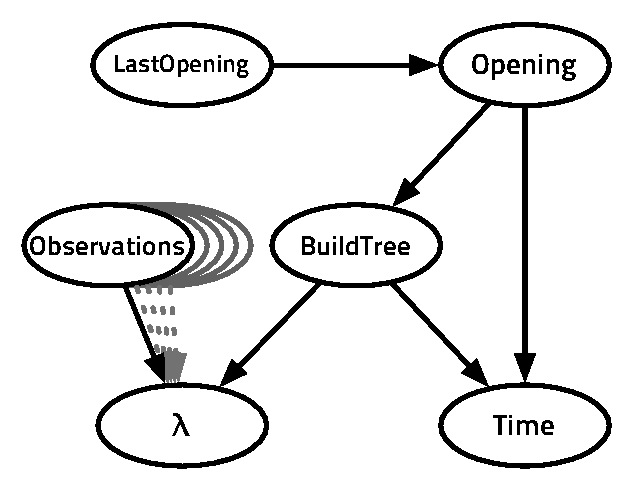
\includegraphics[width=0.4\columnwidth]{images/OpeningPrediction2.pdf}}
%%% \caption{Graph representation of the opening (and tech tree) prediction model}
%%% \label{BNPrediction}
%%% \end{figure}

\subsubsection{Variables}
As before, we have:
\begin{itemize}
\item Build trees: $BT \in [\emptyset, building_1, building_2, building_1\wedge building_2, techtrees, \dots]$: all the possible building trees for the given race. For instance $\{pylon, gate\}$ and $\{pylon, gate, core\}$ are two different $BT$.
\item $N\ $Observations: $O_{i \in \llbracket 1\dots N \rrbracket} \in \{0, 1\}$, $O_k$ is $1\ (true)$ if we have seen (observed) the $k$th building (it can have been destroyed, it will stay ``seen'').
\item Coherence variable: $\lambda \in \{0, 1\}$: coherence variable (restraining $BT$ to possible values with regard to $O_\llbracket 1 \dots N \rrbracket$)
\item Time: $T \in \llbracket 1\dots P \rrbracket$, time in the game (1 second resolution).
\end{itemize}
Additionally, we have:
\begin{itemize}
\item Opening: $Op^t \in [opening_1 \dots opening_M]$ take the various opening values (depending on the race), with opening labels as described in section \ref{sec:openings}.
\item Last opening: $Op^{t-1} \in [opening_1 \dots opening_M]$, opening value of the previous time step (this allows filtering, taking previous inference into account).
\end{itemize}

\subsubsection{Decomposition}
The joint distribution of our model is the following:
\begin{eqnarray}
& & \PP(T, BT, O_1 \dots O_N, Op^t, Op^{t-1}, \lambda) \\ 
& = &   \PP(Op^t | Op^{t-1}) \PP(Op^{t-1}) \PP(BT | Op^t) \PP(T | BT, Op^t) \\
& & \times \PP(\lambda | BT, O_{\llbracket 1 \dots N\rrbracket}) \Pi_{i=1}^N \PP(O_i)
\end{eqnarray}
This can also be seen as Figure~\ref{fig:openingplate}.

\begin{figure}[h]
\centerline{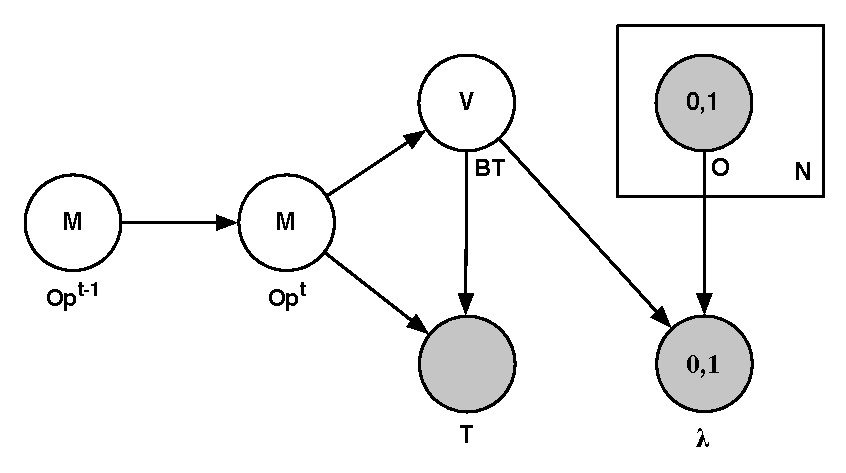
\includegraphics[width=0.7\columnwidth]{images/OpeningPrediction_plate.pdf}}
\caption{Graphical model (plate notation) of the opening Bayesian model, gray variables are known.}
\label{fig:openingplate}
\end{figure}

\subsubsection{Forms}
\begin{itemize}
\item $\PP(Op^t | Op^{t-1})$, we use it as a filter, so that we take into account previous inferences (compressed). 
We use a $Dirac$:
%%% \begin{eqnarray*}
%%% & & \PP(Op^t|Op^{t-1})\ \  (Dirac)\\
%%% & = & 1\ \mathrm{if}\ Op^t = Op^{t-1}\\
%%% & = & 0\ \mathrm{else}
%%% \end{eqnarray*}
\begin{eqnarray*}
\begin{cases}
\PP(Op^t=op^t|Op^{t-1}=op^{t-1}) = 1\ \mathrm{if}\ op^t = op^{t-1}\\
\PP(Op^t=op^t|Op^{t-1}=op^{t-1}) = 0\ \mathrm{else}
\end{cases}
\end{eqnarray*}
This does not prevent our model to switch predictions, it just uses the previous inference's posterior $\PP(Op^{t-1})$ to average $\PP(Op^t)$.

\item $\PP(Op^{t-1})$ is copied from one inference to another (mutated from $\PP(Op^t)$). The first $\PP(Op^{t-1})$ is bootstrapped with the uniform distribution. We could also use a prior on openings in the given match-up, which is directly shown in Tables~\ref{tab:weberdatasetnumbers} and \ref{tab:openings_distrib}.

\item $\PP(BT | Op^t=op)=Categorical(\abs{BT},p_{op})$ is learned from the labeled replays. $\PP(BT|Op^t)$ are $M$ ($\#\{openings\}$) different histogram over the values of $BT$.
\item $\PP(O_{i \in \llbracket 1 \dots N\rrbracket})$ is unspecified, we put the uniform distribution.
\item $\PP(\lambda | BuildTree, O_{\llbracket 1 \dots N\rrbracket})$ is a functional Dirac that restricts $BuildTree$ values to the ones than can co-exist with the observations. As explained above in the build tree model.
%%% \begin{eqnarray*}
%%% & & \PP(\lambda = 1 | buildTree, o_{\llbracket 1 \dots N\rrbracket}) \\
%%% & = & 1\ \mathrm{if\ } buildTree \ \mathrm{can\ exist\ with\ } o_{\llbracket 1\dots N\rrbracket} \\
%%% & = & 0\ \mathrm{else}
%%% \end{eqnarray*}
%%% A $BuildTree$ value ($buildTree$) is compatible with the observations if it covers them fully. For instance, $BuildTree=\{pylon, gate, core\}$ is compatible with $o_{\#core} = 1$ but it is not compatible with $o_{\#forge} = 1$. In other words, $buildTree$ is incompatible with $o_{\llbracket 1\dots N\rrbracket}$ \textit{iff} $\{o_{\llbracket 1\dots N\rrbracket} \backslash \{o_{\llbracket 1\dots N\rrbracket} \wedge buildTree\}\} \neq \emptyset$.

\item $\PP(T | BT=bt, Op^t=op) = \mathcal{N}(\mu_{bt,op},\sigma_{bt,op}^2)$: $\PP(T|BT,Op^t)$ are discrete normal distributions (``bell shapes''). There is one bell shape over $T$ per couple $(opening, buildTree)$. The parameters of these discrete Gaussian distributions are learned from the labeled replays.
\end{itemize}

\subsubsection{Identification (learning)}
The learning of the $\PP(BT | Op^t)$ histogram is straight forward counting of occurrences from the labeled replays with ``add-one smoothing'' (Laplace's law of succession \citep{Jaynes}):
$$\PP(BT=bt|Op^t=op) = \frac{1 + \mathrm{count\_games}(bt\wedge op)}{\abs{BT} + \mathrm{count\_games}(op)}$$

The learning of the $\PP(T | BT, Op^t)$ bell shapes parameters takes into account the uncertainty of the couples $(bt, op)$ for which we have few observations. This is even more important as observations may (will) be sparse for some values of $Op^t$, as can be seen in Figure~\ref{fig:sparseBTOp}. As for the previous, the normal distribution $\PP(T|bt, op)$ begins with a high $\sigma_{bt,op}^2$. This accounts for the fact that the first(s) observation(s) may be outlier(s). %This learning process is independent on the order of the stream of examples, seeing point A and then B or B and then A in the learning phase produces the same result. 

\subsubsection{Questions}
%%%\begin{eqnarray*}
%%%\PP(Op|T=t, O_{1:N}=o_{1:N}, \lambda = 1) \\
%%%\propto \frac{1} {\PP(o_{1:N}).\PP(\lambda).\PP(t)} \\
%%%\sum_{BuildTree} \PP(Op).\PP(BuildTree|Op).\PP(o_{1:N})\\
%%%.\PP(\lambda|BuildTree,o_{1:N}).\PP(t|BuildTree,Op)
%%%\end{eqnarray*}
The question that we will ask in all the benchmarks is:
%%% \begin{eqnarray}
%%%  & \PP(Op|T=t, O_{\llbracket 1\dots N\rrbracket}=o_{\llbracket 1\dots N\rrbracket}, \lambda = 1) \\
%%%  & \propto \PP(Op).\PP(o_{\llbracket 1\dots N\rrbracket})\\
%%%  & \times \sum_{BuildTree} \PP(\lambda | BuildTree, o_{\llbracket 1\dots N\rrbracket})\\
%%%  & .\PP(BuildTree|Op).\PP(t|BuildTree, Op)
%%% \end{eqnarray}
\begin{eqnarray}
 & \PP(Op^t|T=t, O_{\llbracket 1\dots N\rrbracket}=o_{\llbracket 1\dots N\rrbracket}, \lambda = 1) \\
 & \propto \prod_{i=1}^N \PP(o_i) \sum_{Op^{t-1}} \PP(Op^t|Op^{t-1}) \sum_{BT} \PP(\lambda | BT, o_{\llbracket 1\dots N\rrbracket}) \PP(BT|Op^t).\PP(t|BT, Op^t)
\end{eqnarray}
Note that if we see $\PP(BT, Time)$ as a plan, asking $\PP(BT|Op^t, Time)$ boils down to use our ``plan recognition'' mode as a planning algorithm. % which could provide good approximations of the optimal goal set \citep{Ramirez}. 
This gives us a distribution on the build trees to follow (build orders) to achieve a given opening.

\subsubsection{Bayesian program}
%To sum-up, the full Bayesian program is:
\begin{eqnarray*}
\begin{sideways}\parbox{20mm}{\hspace{-1.3cm}Bayesian program}\end{sideways}
\begin{cases}
\begin{sideways}\parbox{15mm}{\hspace{-0.8cm}Description}\end{sideways}
    \begin{cases}
\begin{sideways}\parbox{18mm}{\hspace{-1.1cm}Specification ($\pi$)}\end{sideways}
        \begin{cases}
        Variables\\
    T, BT, O_1 \dots O_N, Op^t, Op^{t-1}, \lambda \\ 
        Decomposition\\
            \PP(T, BT, O_1 \dots O_N, Op^t, Op^{t-1}, \lambda) = JD \\ 
        =   \PP(Op^t | Op^{t-1}) \PP(Op^{t-1}) \PP(BT | Op^t) \\
            %\PP(O_{\llbracket 1 \dots N\rrbracket}) \PP(\lambda | BT, O_{\llbracket 1 \dots N\rrbracket}) \PP(T | BT, Op^t) \\
             \PP(\lambda | BT, O_{\llbracket 1 \dots N\rrbracket}) \PP(T | BT, Op^t) \prod_{i=1}^N\PP(O_{i}) \\
        Forms\\
            \PP(Op^t | Op^{t-1}) = Dirac\ \mathrm{(filtering)}\\
            \PP(Op^t=op^t | Op^{t-1}=op^{t-1}) = 1\ \mathrm{iff}\ op^t==op^{t-1}, 0\ \mathrm{else}\\
            \PP(BT | Op^t=op) = Categorical(\abs{BT}, p_{op})\\
%%% \mathrm{histogram} \\
            \PP(\lambda | BT, O_{\llbracket 1 \dots N\rrbracket}) = functional\ Dirac\ \mathrm{(coherence)}\\ 
%%%\ of\ observations\ with\ buildtree)}\\
            %%%\PP(T | BT, Op^t) = BellShape(\mu, \sigma)
            \PP(T | BT=bt, Op^t=op) = discrete \mathcal{N}(\mu_{bt,op},\sigma^2_{bt,op})\\
%%%\mathrm{bell\ shape\ (discrete\ normal)}\\
        \end{cases}\\
    Identification\\
            \PP(BT=bt | Op^t=op) = \frac{1 + \mathrm{count}(bt,op)}{\abs{BT} + \mathrm{count}(op)}\\
            (\mu_{bt,op},\sigma_{bt,op}) = \argmax_{\mu,\sigma}\PP(T|BT=bt, Op^t=op; \mu,\sigma^2)\\
%%% \mathrm{maximum\ likelihood\ }\{(\mu,\sigma^2)\}\\
    \end{cases}\\
Question \\
 \PP(Op^t|T=t, O_{\llbracket 1\dots N\rrbracket}=o_{\llbracket 1\dots N\rrbracket}, \lambda = 1) \propto \sum_{Op^{t-1}}\sum_{BT} JD \\
\end{cases}
\end{eqnarray*}

\begin{figure}
\centerline{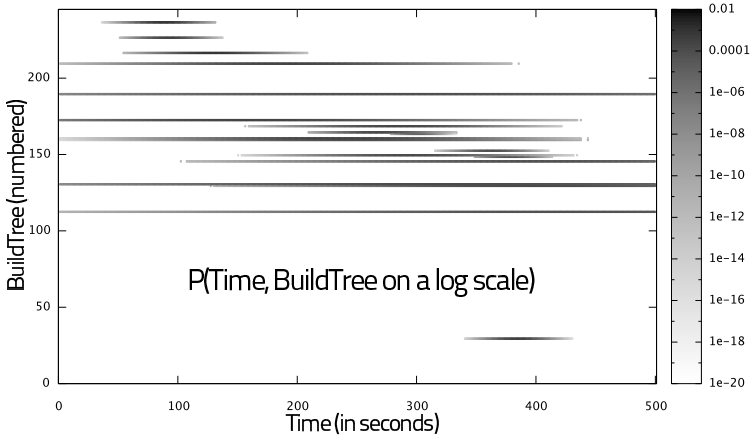
\includegraphics[width=0.82\columnwidth]{images/BW_HeatMap_knowing_ReaverDrop.png}}
\caption{$\PP(T, BT | Op^t=ReaverDrop)$ Values of $BT$ are in y-axis and values of $T$ in x-axis. We have sparse 1-dimensional Gaussian distributions depending on $T$ for each value of $BT$.}
\label{fig:sparseBTOp}
\end{figure}

\subsection{Results}

\subsubsection{Metrics}
For each match-up, we ran cross-validation testing with 9/10th of the dataset used for learning and the remaining 1/10th of the dataset used for testing. We ran tests finishing at 5, 10 and 15 minutes to capture all kinds of openings (early to late ones). To measure the predictive capability of our model, we used 3 metrics: 
\begin{itemize}
\item the \textit{final} prediction, which is the opening that is predicted at the end of the test, 
\item the \textit{online twice} (OT), which counts the openings that have emerged as most probable twice a test (so that their predominance is not due to noise),
\item the \textit{online once} $> 3$ (OO3), which counts the openings that have emerged as most probable openings after 3 minutes (so that these predictions are based on really meaningful information).
\end{itemize}
After 3 minutes, a Terran player will have built his first supply depot, barracks, refinery (gas), and at least factory or expansion. A Zerg player would have his first overlord, zergling pool, extractor (gas) and most of the time his expansion and lair tech. A Protoss player would have his first pylon, gateway, assimilator (gas), cybernectics core, and sometimes his robotics center, or forge and expansion.


\subsubsection{Predictive power}
Table~\ref{tab:openingsresults} sums up all the prediction probabilities (scores) for the most probable opening according to our model (compared to the replay label) in all the match-ups with both labeling of the game logs. The first line should be read as: in the Protoss vs Protoss (PvP) \glos{matchup}, with the rule-based openings labels (Weber's labels), the most probable \glos{opening} (in the $Op$ values) at 5 minutes (``final'') is 65\% correct. The proportion of times that the most probable opening twice (``OT'') in the firsts 5 minutes period was the real one (the game label for this player) is 53\%. The proportion of times that the most probable opening after 3 minutes (``OO3'') and in the firsts 5 minutes periods was the real one is 0.59\%. Then the other columns show the same metrics for 10 and 15 minutes periods, and then the same with our probabilistic clustering.

Note that when an opening is mispredicted, the distribution on openings is often \textbf{not} $\PP(badopening)=1, \PP(others)=0$ and that we can extract some value out of these distributions (see the bot's strategy adaptation in chapter~\ref{chapter:bot}). Also, we observed that $\PP(Opening=unknown)>\PP(others)$ is often a case of misprediction: our bot uses the next prediction in this case. 

\begin{figure}[h]
\centerline{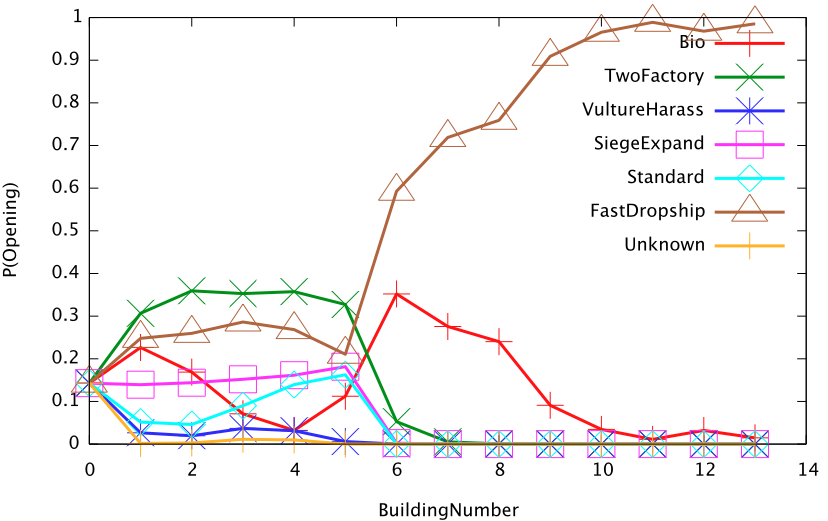
\includegraphics[width=0.7\columnwidth]{images/TvP_prediction.png}}
\centerline{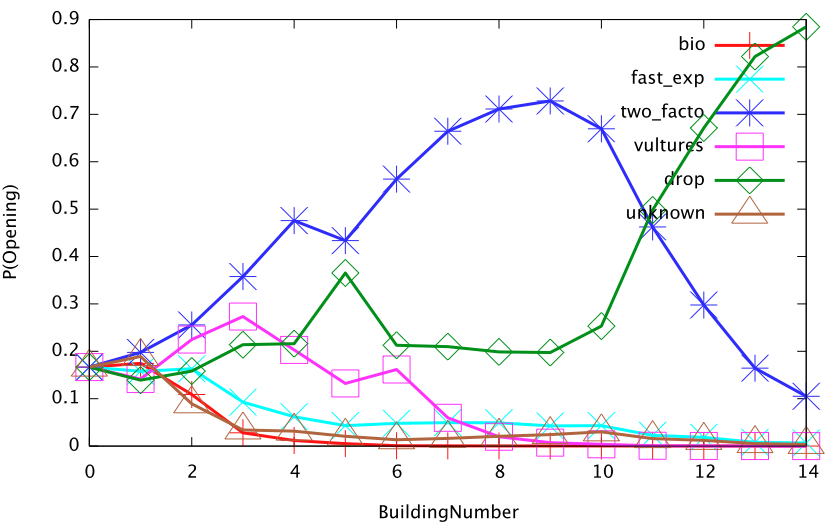
\includegraphics[width=0.7\columnwidth]{images/TvPx_prediction.png}}
\caption{Evolution of $\PP(Opening)$ with increasing observations in a TvP match-up, with Weber's labeling on top, our labeling on the bottom. The x-axis corresponds to the construction of buildings. The interpolation was obtained by fitting a second order polynomial.}
\label{fig:openingsprediction}
\end{figure}

Figure~\ref{fig:openingsprediction} shows the evolutions of the distribution $\PP(Opening)$ during a game for Weber's and our labeling or the openings. We can see that in this game, their \glos{buildtree} and rule-based labeling (top plot) enabled the model to converge faster towards \textit{FastDropship}. With our labeling (bottom plot), the corresponding \textit{drop} opening peaked earlier (5th building vs 6th with their labeling) but it was then eclipsed by \textit{two\_facto} (while staying good second) until later with another key observation (11th building). This may due to unorthodox timings of the \textit{drop} opening, probably because the player was delayed (by a rush, or changed his mind), and that the \textit{two\_facto} opening has a larger (more robust to delays) support in the dataset.

\subsubsection{Robustness to noise}

Figure~\ref{fig:openingsnoise} shows the resistance of our model to noise. We randomly removed some observations (buildings, attributes), from 1 to 15, knowing that for Protoss and Terran we use 16 buildings observations and 17 for Zerg. We think that our model copes well with noise because it backtracks unseen observations: for instance if we have only the $core$ observation, it will work with build trees containing $core$ that will passively infer unseen $pylon$ and $gate$. 


\begin{figure}[h]
\centerline{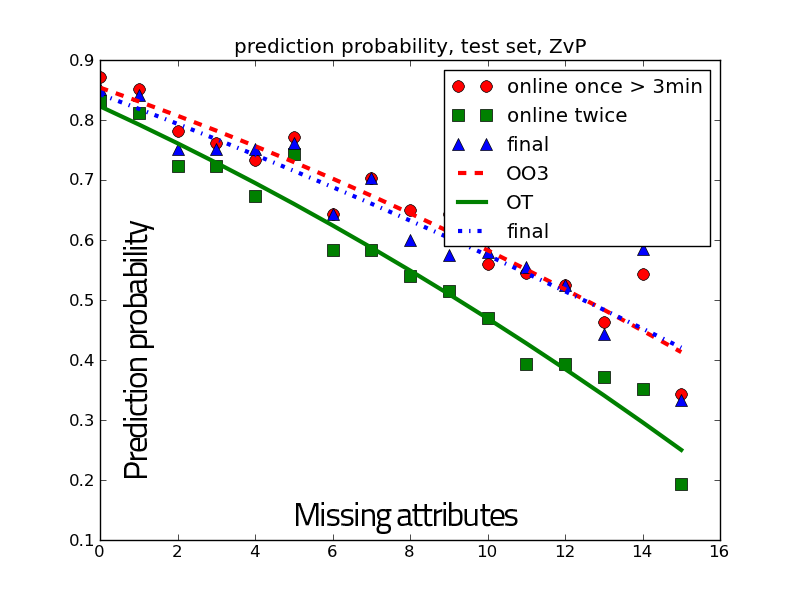
\includegraphics[width=0.7\columnwidth]{images/ZvP2.png}}
\centerline{\includegraphics[width=0.7\columnwidth]{images/PvZ2.png}}
\caption{Two extreme evolutions of the 3 probabilities of opening recognition with increasing noise (15 missing attributes/observations/buildings correspond to 93.75\% missing information for Protoss and Terran openings prediction and 88.23\% of missing attributes for Zerg openings prediction). Zerg opening prediction probabilitly on top, Protoss bottom.}
\label{fig:openingsnoise}
\end{figure}

\begin{sidewaystable}
\caption{Prediction probabilities for all the match-ups, at 5 minutes, 10 minutes, 15 minutes, both for Weber's labels and for our labels. The three metrics are 1) final: what is the most probable at the end of the time equals compared to the label, 2) OT: (online twice) what was the most probable in two different inferences during the game compared to the label, 3) OO3 (online once > 3 minutes) what was the most probable opening after 3 minutes of game compared to the label.}
%\caption{Prediction probabilities for all the match-ups, at 5 minutes, 10 minutes, 15 minutes, both for Weber's labels and for our labels. The three metrics are: final: 1 if what is the most probable at the end of the time limit equals the label, else 0; OT: (online twice) 1 if what was the most probable in two different inferences during the game equals the label, else 0; OO3 (online once > 3 minutes) 1 if what was the most probable opening after 3 minutes of game was equal to the label, else 0.}
\begin{center}
\begin{tabular}{|c|ccc|ccc|ccc|ccc|ccc|ccc|}
\hline
& \multicolumn{9}{|c|}{Weber and Mateas' labels}
& \multicolumn{9}{|c|}{Our labels}
\\  \hline
& \multicolumn{3}{|c|}{5 minutes}
& \multicolumn{3}{|c|}{10 minutes}
& \multicolumn{3}{|c|}{15 minutes}
& \multicolumn{3}{|c|}{5 minutes}
& \multicolumn{3}{|c|}{10 minutes}
& \multicolumn{3}{|c|}{15 minutes}
\\
\begin{scriptsize}match-up\end{scriptsize}
& final
& OT
& OO3
& final
& OT
& OO3
& final
& OT
& OO3
& final
& OT
& OO3
& final
& OT
& OO3
& final
& OT
& OO3 \\ \hline
PvP & 0.65 & 0.53 & 0.59 & 0.69 & 0.69 & 0.71 & 0.65 & 0.67 & 0.73
& 0.78 & 0.74 & 0.68 & 0.83 & 0.83 & 0.83 & 0.85 & 0.83 & 0.83 \\
PvT & 0.75 & 0.64 & 0.71 & 0.78 & 0.86 & 0.83 & 0.81 & 0.88 & 0.84
& 0.62 & 0.69 & 0.69 & 0.62 & 0.73 & 0.72 & 0.6 & 0.79 & 0.76 \\
PvZ & 0.73 & 0.71 & 0.66 & 0.8 & 0.86 & 0.8 & 0.82 & 0.87 & 0.8
& 0.61 & 0.6 & 0.62 & 0.66 & 0.66 & 0.69 & 0.61 & 0.62 & 0.62 \\
TvP & 0.69 & 0.63 & 0.76 & 0.6 & 0.75 & 0.77 & 0.55 & 0.73 & 0.75
& 0.50 & 0.47 & 0.54 & 0.5 & 0.6 & 0.69 & 0.42 & 0.62 & 0.65 \\
TvT & 0.57 & 0.55 & 0.65 & 0.5 & 0.55 & 0.62 & 0.4 & 0.52 & 0.58
& 0.72 & 0.75 & 0.77 & 0.68 & 0.89 & 0.84 & 0.7 & 0.88 & 0.8 \\
TvZ & 0.84 & 0.82 & 0.81 & 0.88 & 0.91 & 0.93 & 0.89 & 0.91 & 0.93
& 0.71 & 0.78 & 0.77 & 0.72 & 0.88 & 0.86 & 0.68 & 0.82 & 0.81 \\
ZvP & 0.63 & 0.59 & 0.64 & 0.87 & 0.82 & 0.89 & 0.85 & 0.83 & 0.87
& 0.39 & 0.56 & 0.52 & 0.35 & 0.6 & 0.57 & 0.41 & 0.61 & 0.62 \\
ZvT & 0.59 & 0.51 & 0.59 & 0.68 & 0.69 & 0.72 & 0.57 & 0.68 & 0.7
& 0.54 & 0.63 & 0.61 & 0.52 & 0.67 & 0.62 & 0.55 & 0.73 & 0.66 \\
ZvZ & 0.69 & 0.64 & 0.67 & 0.73 & 0.74 & 0.77 & 0.7 & 0.73 & 0.73
& 0.83 & 0.85 & 0.85 & 0.81 & 0.89 & 0.94 & 0.81 &  0.88 & 0.94\\ \hline
\begin{scriptsize}overall\end{scriptsize} & 0.68 & 0.62 & 0.68 & 0.73 & 0.76 & 0.78 & 0.69 & 0.76 & 0.77 
& 0.63 & 0.67 & 0.67 & 0.63 & 0.75 & 0.75 & 0.63 & 0.75 & 0.74 \\ \hline
\end{tabular}
\label{tab:openingsresults}
\end{center}
\end{sidewaystable}


\subsubsection{Computational performances}
The first iteration of this model was not making use of the structure imposed by the game in the form of ``possible build trees'' and was at best very slow, at worst intractable without sampling. With the model presented here, the performances are ready for production as shown in Table~\ref{CPU}. The memory footprint is around 3.5Mb on a 64bits machine. Learning computation time is linear in the number of games logs events ($O(N)$ with $N$ observations), which are bounded, so it is linear in the number of game logs. It can be serialized and done only once when the dataset changes. The prediction computation corresponds to the sum in the question (III.B.5) and so its computational complexity is in $O(N\cdot M)$ with $N$ build trees and $M$ possible observations, as $M << N$, we can consider it linear in the number of build trees (values of $BT$).

\begin{table}[h]
\caption{Extremes of computation time values (in seconds, Core 2 Duo 2.8Ghz)}
\begin{center}
\begin{tabular}{|c|cc|cc|}
\hline
Race
& Nb Games
& Learning time
& Inference $\mu$
& Inference $\sigma^2$ \\ \hline
T (max) & 1036 & 0.197844 & 0.0360234 & 0.00892601 \\
T \begin{tiny}(Terran)\end{tiny} & 567 & 0.110019 & 0.030129 & 0.00738386 \\ 
P \begin{tiny}(Protoss)\end{tiny} & 1021 & 0.13513 & 0.0164457 & 0.00370478 \\
P \begin{tiny}(Protoss)\end{tiny} & 542 & 0.056275 & 0.00940027 & 0.00188217 \\ 
Z \begin{tiny}(Zerg)\end{tiny} & 1028 & 0.143851 & 0.0150968 & 0.00334057 \\
Z \begin{tiny}(Zerg)\end{tiny} & 896 & 0.089014 & 0.00796715 & 0.00123551 \\ \hline
\end{tabular}
\label{CPU}
\end{center}
\end{table}

\subsubsection{Strengths and weaknesses of StarCraft openings}
\label{sec:openingsstrengthsweaknesses}

We also proceeded to analyze the strengths and weaknesses of openings against each others. For that, we labeled the dataset with openings and then learned the $\PP(Win=true|Op_{player1}^t,Op_{player2}^t)$ probability table with Laplace's rule of succession. As can be seen in Table~\ref{tab:weberdatasetnumbers}, not all openings are used for one race in each of its 3 \gloss{matchup}. Table~\ref{table:openingcontingency} shows some parts of this $\PP(Win=true|Op_{player1}^t,Op_{player2}^t)$ ratios of wins for openings against each others. This analysis can serve the purpose of choosing the right opening as soon as the opponent's opening was inferred.

\begin{table}[h] 
\begin{center}
\begin{small}
\begin{tabular}{|l|ccccc|}
\hline
\begin{tiny}Zerg | Protoss\end{tiny} & two gates & fast dt & reaver drop & corsair & nony\\
\hline
speedlings &  0.417& 0.75 & NED & NED & 0.5 \\
lurkers &  NED & 0.493& NED & 0.445 & 0.533\\
fast mutas &  NED & 0.506& 0.5 & 0.526& 0.532\\
\hline
\end{tabular}
\begin{tabular}{|l|cccc|}
\hline
\begin{tiny}Terran | Protoss\end{tiny} & fast dt & reaver drop & corsair & nony\\
\hline
%%% bio &  NED & NED & NED & NED & NED & NED \\
%%% unknown &  NED & NED & 0.5 & NED & NED & NED \\
%%% drop &  NED & NED & NED & NED & NED & NED \\
two facto &  0.552& 0.477& NED & 0.578\\
rax fe &  0.579& 0.478& 0.364& 0.584\\
%%% vultures &  NED & NED & NED & NED & NED & NED \\
\hline
\end{tabular}
\end{small}
\caption{Opening/Strategies labels counted for victories against each others for the PvZ (top, on 1408 games) and PvT (bottom, on 1657 games) match-ups. NED stands for Not Enough Data to conclude a preference/discrepancy towards one opening. The results should be read as win rates of columns openings vs lines openings.}
\end{center}
\label{table:openingcontingency}
\end{table}

\subsection{Possible uses}
%%% We recall how we used this whole model:
%%% \begin{itemize}
%%%     \item for build trees or tech trees prediction, as a proxy for the estimation of an opponent's technologies and production capabilities.
%%%     \item for opening prediction, as a proxy for timing attacks and aggressiveness.
%%% \end{itemize}
We recall that we used this model for opening prediction, as a proxy for timing attacks and aggressiveness. It can also be used:
\begin{itemize}
    \item for build tree suggestion when wanting to achieve a particular opening. Particularly one does not have to encode all the openings into a finite state machine: simply train this model and then ask $\PP(BT|time,opening,\lambda=1)$ to have a distribution on the build trees that generally are used to achieve this $opening$.
    \item as a commentary assistant AI. In the StarCraft and StarCraft 2 communities, there are a lot of progamers tournaments that are commented and we could provide a tool for commentators to estimate the probabilities of different openings or technology paths. As in commented poker matches, where the probabilities of different hands are drawn on screen for the spectators, we could display the probabilities of openings. In such a setup we could use more features as the observers and commentators can see everything that happens (upgrades, units) and we limited ourselves to ``key'' buildings in the work presented here.
\end{itemize}

\subsubsection{Possible improvements}
\label{sec:openingspossibleimprovements}

First, our prediction model can be upgraded to explicitly store transitions between $t$ and $t+1$ (or $t-1$ and $t$) for openings ($Op$) and for \gloss{buildtree} ($BT$). The problem is that $\PP(BT^{t+1}|BT^t)$ will be very sparse, so to efficiently learn something (instead of a sparse probability table) we have to consider a smoothing over the values of $BT$, perhaps with the distances mentioned in section~\ref{sec:buildtreemetrics}. If we can learn $\PP(BT^{t+1}|BT^t)$, it would perhaps increase the results of $\PP(Opening|Observations)$, and it almost surely would increase $\PP(BuildTree^{t+1}|Observations)$, which is important for late game predictions. 

Incorporating $\PP(Op^{t-1})$ priors per match-up (from Table~\ref{tab:weberdatasetnumbers}) would lead to better results, but it would seem like overfitting to us: particularly because we train our robot on games played by humans whereas we have to play against robots in competitions.

%We could also make use of more features as we currently only use at most 20 features (only buildings), and never all at once. 
%TODO

%Then, we could feed it with \textit{more} replays during the learning by scrapping more progamers level replays websites. Also, we could learn from replays of bot vs bot matches. For the learning part, the labeling of replays is very important, and our labeling methods can be improved. 
%We could explore auto-supervised learning \citep{AutoSuperLearning}. 
Clearly, some match-ups are handled better, either in the replays labeling part and/or in the prediction part. Replays could be labeled by humans and we would do supervised learning then. Or they could be labeled by a combination of rules (as in \citep{weberStrat}) and statistical analysis (as the method presented here). Finally, the replays could be labeled by match-up dependent openings (as there are different openings usages by \gloss{matchup}, see Table~\ref{tab:weberdatasetnumbers}), instead of race dependent openings currently. The labels could show either the two parts of the opening (early and late developments) 
or the game time at which the label is the most relevant, as openings are often bimodal (``fast expand into mutas'', ``corsairs into reaver'', etc.).

Finally, a hard problem is detecting the ``fake'' builds of very highly skilled players. Indeed, some progamers have build orders which purpose are to fool the opponent into thinking that they are performing opening A while they are doing B. For instance they could ``take early gas'' leading the opponent to think they are going to do tech units, not gather gas 
%For instance, they could lead the opponent to think they are going to \textit{tech} 
and perform an early rush instead. We think that this can be handled by our model by changing $\PP(Opening|LastOpening)$ by $\PP(Opening|LastOpening, LastObservations)$ and adapting the influence of the last prediction with regard to the last observations (i.e., we think we can learn some ``fake'' label on replays). If a player seem on track to perform a given opening but fails to deliver the key characteristic (heavy investment, timing attack...) of the opening, this may be a fake.
%\subsubsection{Partial Conclusion}


\section{Army composition}
\label{sec:armycomposition}
We reuse the predictions on the \glos{buildtree} ($\PP(BT)$) directly for the \glos{techtree} ($\PP(TT)$) (for the enemy, so $ETT$) by estimating $BT$ as presented above and simply adding the tech tree additional features (upgrades, researches) that we already saw\footnote{We could also modify the models above and incorporate tech tree features but it is of little benefit. Also, $BT$ contains duplicates of buildings and is it easier to downgrade to $TT$ than to estimate the openings from $TT$ instead of $BT$.}. You can just assume that $BT=TT$, or refer to section~\ref{sec:buildings}.

\subsection{Bayesian model}

In this model, we assume that we have some incomplete knowledge of the opponent's tech tree and a quite complete knowledge of his army composition. We want to know what units we should build now, to adapt our army to their, while staying coherent with our own tech tree and tactics constraints. To that end, we reduce armies to mixtures of clusters that could have generated a given composition. In this lower dimension (usually between 5 to 15 mixture components), %, up to 50 ``hard'' clusters), 
we can reason about which mixture of clusters the opponent is probably going to have, according to his current mixture components and his tech tree. As we learned how to pair compositions strengths and weaknesses, we can adapt to this ``future mixture''. %This Bayesian program can be seen as the Bayesian network represented in Figure~\ref{fig:armycompositionplate}. %It is a generative model and this helps dealing with the parts of the observations' space where we do not have too much data (RTS games tend to diverge from one another as the number of possible actions grow exponentially), as generative models tend to converge with fewer observations than discriminative ones \cite{Jordan}. Here is the description of our Bayesian program:

\subsubsection{Variables}
\begin{itemize}
    %\item $BT^t$ is a \glos{buildtree}\footnote{with an exception for the Zerg Lurker, which requires a research, we can know all the units types that it is possible to train/recruit/product this way.} variable, at time $t$. $BT \in \{\emptyset, \{building_1\}, \{building_2\}, \{building_1\wedge building_2\},$ $\dots\}$: all the possible building trees for the given race ). For instance $\{pylon, gate\}$ and $\{pylon, gate, core\}$ are two different $TechTrees$. $TT$ has $V$ possible values and $ETT$ has $V'$ possible values (depending on the faction).
    \item $TT^t$ is a \glos{techtree} variable, at time $t$. $TT \in \{\emptyset, \{building_1\}, \{building_2\}, \{building_1\wedge building_2\},$ $\dots\}$: all the possible building trees for the given race. %Strictly speaking, we here only use build tree $\cap$ tech tree: 
We just want to know what unit types we can produce and not recreate the whole technological state. %For instance $\{pylon, gate\}$ and $\{pylon, gate, core\}$ are two different $TechTrees$. 
$TT$ has $V$ possible values ($V$ is the number different \gloss{techtree} and depends on the faction).

    \item $ETT^t$ the enemy tech tree, same as above but for the enemy. $ETT$ has $V'$ possible values.

    \item $EC^{t,t+1} \in \{enemy's\ race's\ clusters\}$ the enemy's cluster ($EC$) estimated at $t$ from their units that we saw, and estimated at $t+1$ from their (estimated distribution on) tech trees ($ETT$) and previous $EC^t$. $EC^t, EC^{t+1}$ each have $K'$ values (number of mixtures components).

    \item $C_{t,c,m,f}^{t+1} \in \{our\ race's\ clusters\}$, our army cluster ($C$), both wanted ($C_{t}$ for $tactics$,$C_{c}$ for $counter$, $C_{m}$ for $merge$) and decided ($C_{f}$ for $final$) at $t+1$. $C_{t},C_{c},C_{m},C_{f}$ have $K$ values ($K$ units clusters for us). 
We infer $C_c$ the ``counter'' cluster for (adaptation to) $EC^{t+1}$. $C_t$ (a distribution $C_t$) comes from the needs of specific units by the tactical model, we merge $C_t$ and $C_c$ in $C_m$ (merge). The final clusters ($C_f$) corresponds to what is coherent with our tech tree ($TT$) so use a coherence variable ($\lambda$) to make $C_m$ and $C_f$ coherent. See Figure~\ref{fig:armycompositionplate}.
%$C_t$ is %a distribution of 
%the cluster we want for tactics. % or just a value (for instance we just need a \textit{dropship/shuttle}). 
%$C_c$ is the counter to what we infer the enemy army will be ($EC^{t+1}$). 
%$C_m$ merge our tactics desiderata ($C_t$) with our adaptability ($C_c$), 
%while $C_f$ take the tech tree constraints into account. This can seem tedious but these variables are all to be seen as different states of $C$, representing our army composition.

    \item $U^{t+1} \in ([0,1]\dots[0,1])$, our $N$ dimensional unit types ($U$) proportions at time $t+1$, i.e. $U^{t+1} \in [0,1]^N$. For instance, an army with equal numbers of $zealots$ and $dragoons$ (and nothing else) is represented as $\{U_{zealot}=0.5, U_{dragoon}=0.5, \forall ut \neq zealot|dragoon\ U_{ut}=0.0\}$, i.e. $U=(0.5,0.5,0,\dots,0)$ if $zealots$ and $dragoons$ are the first two components of the $U$ vector. So $\sum_i U_i = 1$ whatever the composition of the army.

    \item $EU^t$ and $EU^{t+1} \in ([0,1]\dots [0,1])$, the $M$ enemy units types ($EU$) at time $t$ and $t+1$, i.e. $EU^t \in [0,1]^M$. Same as above, but for the enemy and at two different times ($t$ and $t+1$).

    \item $\lambda \in \{0, 1\}$ is a coherence variable unifying $C_{m}^{t+1}$ and $C_{f}^{t+1}$ to possible values with regard to $TT^t$.

\end{itemize}

For tech trees ($TT$ and $ETT$) values, it would be absurd to generate all the possible combinations, exactly as for $BT$ (see the previous two sections). We use our previous $BT$ and the researches. % (for instance no player is going to build four barracks before building the first supply depot), we used all the values that were encountered in our games (replays) dataset. The bases of these trees were buildings, with some types being counted for repetition, for instance a tech tree of $\{pylon, gateway\}$ is not the same as $\{pylon, gateway, gateway\}$: we effectively count the gateway twice. %We added multiple instances of the basic unit producing buildings (gateway, barracks, hatchery), expansions and supply buildings (depot, pylon, ``overlord'' as a building). 
This way, we counted 273 probable tech tree values for Protoss, 211 for Zerg, and 517 for Terran (the ordering of add-on buildings is multiplying tech trees for Terran). Should it happen, we can deal with unseen tech tree either by using the closest one (in set distance) or using an additional value of no knowledge. %See \cite{SYNNAEVE:StratPred} (which deals with build trees, $BT$) for more details on inferring tech trees.

\subsubsection{Decomposition}
The joint distribution of our model is the following:
\begin{eqnarray}
%%% & & \PP(TT^t,C_{t}^{t+1},C_{c}^{t+1},C_{m}^{t+1},C_{f}^{t+1},ETT^t,EC^{t},EC^{t+1},U_{1:N}^{t+1},EU_{1:M}^{t}) \\
%%% & = & \PP(EU_{1:M}^t|EC^t)\PP(EC^t|EC^{t+1})\PP(EC^{t+1}|ETT^t)\PP(ETT^t)\\
%%% & & \times \PP(C_{c}^{t+1}|EC^{t+1})\PP(C_{t}^{t+1})\PP(TT^t)\PP(C_{f}^{t+1}|TT^{t})\\
%%% & & \times \PP(\lambda|C_{f}^{t+1},C_{m}^{t+1})\PP(C_{m}^{t+1}|C_{t}^{t+1},C_{c}^{t+1}) \PP(U_{1:N}^{t+1}|C_{f}^{t+1})
& & \PP(TT^t,C_{t}^{t+1},C_{c}^{t+1},C_{m}^{t+1},C_{f}^{t+1},ETT^t,EC^{t},EC^{t+1},U^{t+1},EU^{t}) \\
& = & \PP(EU^t|EC^t)\PP(EC^t|EC^{t+1})\PP(EC^{t+1}|ETT^t)\PP(ETT^t)\\
& & \times \PP(C_{c}^{t+1}|EC^{t+1})\PP(C_{t}^{t+1})\PP(C_{m}^{t+1}|C_{t}^{t+1},C_{c}^{t+1}) \\
& & \times \PP(\lambda|C_{f}^{t+1},C_{m}^{t+1})\PP(C_{f}^{t+1}|TT^{t})\PP(TT^t)\PP(U^{t+1}|C_{f}^{t+1})
\end{eqnarray}
This can also be see as Figure~\ref{fig:armycompositionplate}.
\begin{figure}[h]
\centerline{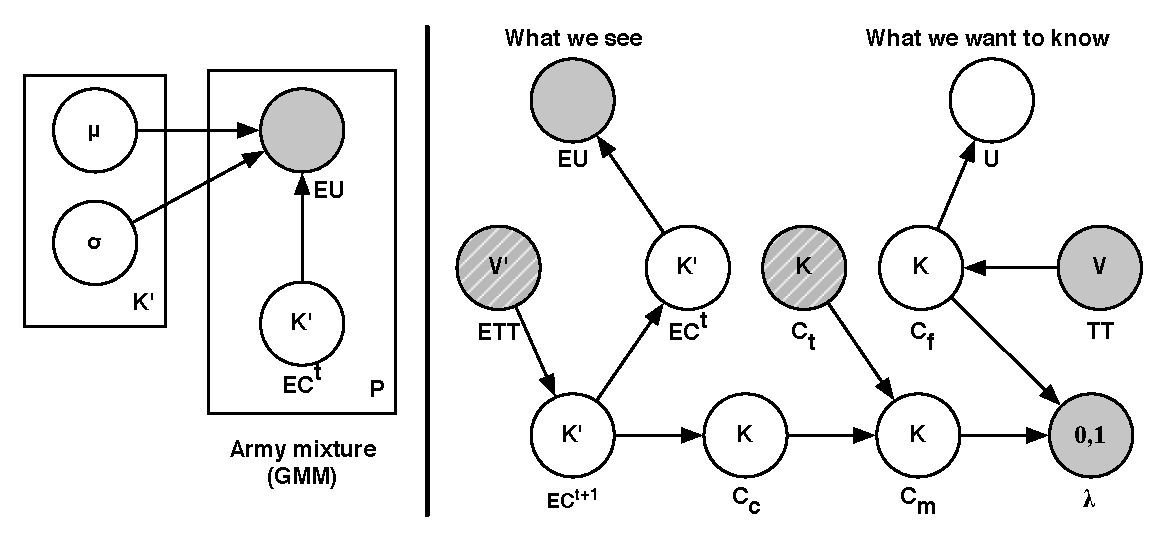
\includegraphics[width=0.84\columnwidth]{images/army_composition_model3.pdf}}
\caption{Left: the full Gaussian mixture model for Q armies (Q battles) for the enemy, with $K'$ mixtures components. Right: Graphical (plate notation) representation of the army composition Bayesian model, gray variables are known while for gray hatched variables we have distributions on their values. $C_t$ can also be known (if a decision was taken at the tactical model level).}
\label{fig:armycompositionplate}
\end{figure}

\subsubsection{Forms}
\begin{itemize}
%%% \item $\PP(U^{t+1}|C_f^{t+1}=c) = \PP(U_{1:N}^{t+1}|C_f^{t+1}=c) = \mathcal{N}(\mu_{c},\sigma_{c}^2)$, the $\mu$ and $\sigma$ come from a Gaussian mixture model learned from all the battles in the dataset (see left diagram on Fig.~\ref{fig:armycompositionplate} and section~\ref{GMMEM}). 
%%% \item $\PP(EU^t | EC^t=ec) = \PP(EU_{1:M}^t|EC^t=ec) = \mathcal{N}(\mu_{ec},\sigma{ec}^2)$, as above but with different parameters for the enemy's race (if it is not a mirror match-up).
\item $\PP(EU^t | EC^t=ec) = \mathcal{N}(\mu_{ec},\sigma{ec}^2)$, as above but with different parameters for the enemy's race (if it is not a mirror match-up).

\item $\PP(EC^t|EC^{t+1}=ec^{t+1}) = Categorical(K',p_{ec^{t+1}})$, $\PP(EC^t|EC^{t+1})$ is a probability table of dimensions $K' \times K'$ resulting of the temporal dynamic between clusters, that is learned from the dataset with a soft Laplace's law of succession (``add one'' smoothing) \cite{Jaynes}. 

\item $\PP(EC^{t+1}|ETT^t=ett) = Categorical(K',p_{ett})$, $\PP(EC^{t+1}|ETT^t)$ is a probability table of dimensions $K' \times V'$ resulting of the inter-dependency between some tech trees and clusters/mixtures. It is learned from the dataset with a soft Laplace's law of succession.

\item $\PP(ETT^t) = Categorical(V',p_{eracett})$, it is a categorical distribution on $V'$ values, i.e. an histogram distribution on the enemy's tech trees. It comes from the build/tech tree prediction model explained above (section~\ref{sec:strategyprediction}). For us, $TT \sim Categorical(V)$ too, and we know our own tech tree ($TT$) exactly.

\item $\PP(C_c^{t+1}|EC^{t+1}=ec) = Categorical(K,p_{ec})$, $\PP(C_c^{t+1}|EC^{t+1})$ is a probability table of dimensions $K \times K'$, which is learned from battles with a soft Laplace's law of succession on victories. 

\item $\PP(C_t^{t+1}) = Categorical(K,p_{tac})$ (histogram on the $K$ clusters values) coming from the tactical model. Note that it can be degenerate: $\PP(C_t^{t+1}=shuttle)=1.0$. It serves the purpose of merging tactical needs with strategic ones.

%\item $\PP(C_m^{t+1}|C_t^{t+1},C_c^{t+1})$
\item $\PP(C_m^{t+1}|C_t^{t+1},C_c^{t+1}) = \alpha \PP(C_t^{t+1})+(1-\alpha) \PP(C_c^{t+1})$ with $\alpha \in [0\dots1]$ the aggressiveness/initiative parameter which can be set fixed, learned, or be variable ($P(\alpha|situation)$). If $\alpha=1$ we only produce units wanted by the tactical model, if $\alpha=0$ we only produce units that adapts our army to the opponent's army composition.

\item $\PP(\lambda | C_f^{t+1},C_m^{t+1})$ is a functional $Dirac$ that restricts $C_m$ values to the ones that can co-exist with our tech tree ($C_f$).
\begin{eqnarray*}
& & \PP(\lambda = 1 | C_f, C_m=c_m) \\
& = & 1\ \mathrm{iff\ } \PP(C_f=c_m) \neq 0\\
& = & 0\ \mathrm{else}
\end{eqnarray*}
This was simply implemented as a function. This is not strictly necessary (as one could have $\PP(C_f|TT,C_m)$ which would do the same for $\PP(C_f)=0.0$) but it allows us to have the same table form for $\PP(C_f|TT)$ than for $\PP(EC|ETT)$, should we wish to use the learned co-occurrences tables (with respect to the good race).

\item $\PP(C_f^{t+1}|TT)$ is either a learned probability table, as for $P(EC^{t+1}|ETT^t)$, or a functional $Dirac$ distribution which tells which $C_f$ values ($c_f$) are compatible with the current tech tree $TT=tt$. We used this second option. A given $c$ is compatible with the tech tree ($tt$) if it allows for building all units present in $c$. For instance, $tt=\{pylon, gate, core\}$ is compatible with a $c=\{\mu_{U_{zealot}}=0.5, \mu_{U_{dragoon}}=0.5, \forall ut \neq zealot|dragoon\ \mu_{U_{ut}}=0.0\}$, but it is not compatible with $c'=\{\mu_{U_{arbiter}}=0.1, \dots\}$.

\item $\PP(U^{t+1}|C_f^{t+1}=c) = \mathcal{N}(\mu_{c},\sigma_{c}^2)$, the $\mu$ and $\sigma$ come from a Gaussian mixture model learned from all the battles in the dataset (see left diagram on Fig.~\ref{fig:armycompositionplate} and section~\ref{GMMEM}). 



\end{itemize}

\subsubsection{Identification (learning)}
%The first approach to clustering units was a simple fusion $\PP(U_{1:N},C)\propto \prod_i \PP(U_i|C)$ with rectangular $\PP(U_i|C)$ distributions above thresholds for basic and special (casters) units, and their compositions. So we fixed $\approx 8+4+4*8 = 44$ clusters (for each race) and set their parameters. The problem with this approach is that it requires a high game strategy expertize and understanding of the multiple influences of parameters, while it cannot take into account singular combinations of 3 (or more) unit types. 
We learned Gaussian mixture models (GMM) with the expectation-maximization (EM) algorithm on 5 to 15 mixtures with spherical, tied, diagonal and full co-variance matrices \cite{scikit-learn}. We kept the best scoring models according to the Bayesian information criterion (BIC) \cite{schwarz1978}. % $-2 \ln{\max{Likelihood}} + k \ln(n)$, with $k$ the number of parameters and $n$ the number of observations. %used the python library scikit-learn  to learn the Gaussian Mixture Models. 

\begin{itemize}
    \item $\PP(U^{t+1}|C_f^{t+1}=c)$ is the result of the clustering of the armies compositions ($U$) into $C$, and so depends from the clustering model. 
%In the best model that we tried, they come from a Gaussian mixtures model (GMM) and so are from $\mathcal{N}(\mu_{z_i}, \sigma^2_{z_i})$ with $z_i \sim Categorial(K)$, respectively $Categorical(K')$.
In our implementation, $\mu_{c},\sigma_{c}$ are learned from the data through expectation maximization. One can get a good grasp on this parameters by looking at Figure~\ref{fig:parallelplot}.
%%% TODO GMM EM

    \item It is the same for $\mu_{ec},\sigma_{ec}$, they are learned by EM on the dataset (see section~\ref{GMMEM}).

    \item $\PP(EC^t=ec^t|EC^{t+1}=ec^{t+1}) = \frac{1+ \PP(ec^t)\PP(ec^{t+1}) \times \mathrm{count}(ec^t \rightarrow ec^{t+1})}{K+\PP(ec^{t+1})\times \mathrm{count}(ec^{t+1})}$

    \item $\PP(ETT^t)$ comes from the model described two sections above (\ref{sec:techtreepred}).

    \item $\PP(EC^{t+1}=ec|ETT^t=ett) = \frac{1 + \PP(ec) \times \mathrm{count}(ec \wedge ett)}{K' + \mathrm{count}(ett)}$

    \item $\PP(C_c^{t+1}=c | EC^{t+1}=ec) = \frac{1 + \PP(c)\PP(ec) \times \mathrm{count_{battles}}(c > ec)}{K + \PP(ec)\mathrm{count_{battles}}(ec)}$, we only count when $c$ won against $ec$.
    
    \item Both $\PP(C_f^{t+1}|TT)$ and $\PP(\lambda | C_f^{t+1},C_m^{t+1})$ are functions and do not need identification.

%We also implemented other clustering methods and variants which are listed in the benchmark.
%$\PP(c_c|ec) = \frac{n_{victories}(c_c, ec)+1}{n_{battles}(c_c, ec)+K}$.

\end{itemize}


\subsubsection{Questions}
The question that we ask to know which units to produce is:
\begin{eqnarray}
 & & \PP(U^{t+1} | eu^t, tt^t, \lambda = 1) \\
 & \propto & \sum_{ETT^t, EC^t, EC^{t+1}}\Big[\PP(EC^{t+1}|ETT^t)\PP(ETT^t)\\
 & & \times \PP(eu^t|EC^t) \sum_{C_f^{t+1},C_m^{t+1},C_c^{t+1},C_t^{t+1}}\big[\PP(C_c^{t+1}|EC^{t+1})\\
 & & \times \PP(C_{t}^{t+1})\PP(C_{f}^{t+1}|tt^{t}) \PP(\lambda|C_{f}^{t+1},C_{m}^{t+1}) \PP(U^{t+1}|C_f^{t+1})\big]\Big]
\end{eqnarray}
or we can sample $U^{t+1}$ from $P(C_f^{t+1})$ or even from $c_f^{t+1}$ (a realization of $C_f^{t=1}$) if we ask $\PP(C_f^{t+1} | eu_{1:M}^t, tt^t, \lambda = 1)$. Note that here we do not know fully neither the value of $ETT$ nor of $C_t$ so we take the most information that we have into account (distributions). The evaluation of the question is proportional to $\abs{ETT}\times \abs{EC}^2\times |C|^4 = V'\times K'^2 \times K^4$. But we do not have to sum on the 4 types of $C$ in practice: $\PP(C_m|C_t,C_c)$ is a simple linear combination of vectors and $\PP(\lambda=1|C_f,C_m)$ is a linear filter function, so we just have to sum on $C_c$ and practical complexity is proportional to $V'\times K'^2 \times K$. As we have most often $\approx 10$ Gaussian components in our GMM, $K$ or $K'$ are in the order of 10 (5 to 12 in practice), while $V$ and $V'$ are between 211 and 517 as noted above.

\subsubsection{Bayesian program}

\begin{eqnarray*}
\begin{sideways}\parbox{20mm}{\hspace{-1.3cm}Bayesian program}\end{sideways}
\begin{cases}
\begin{sideways}\parbox{15mm}{\hspace{-0.8cm}Description}\end{sideways}
    \begin{cases}
\begin{sideways}\parbox{18mm}{\hspace{-1.1cm}Specification ($\pi$)}\end{sideways}
        \begin{cases}
        Variables\\
            TT^t,C_{t}^{t+1},C_{c}^{t+1},C_{m}^{t+1},C_{f}^{t+1},ETT^t,EC^{t},EC^{t+1},U^{t+1},EU^{t}\\
        Decomposition\\
            \PP(TT^t,C_{t}^{t+1},C_{c}^{t+1},C_{m}^{t+1},C_{f}^{t+1},ETT^t,EC^{t},EC^{t+1},U^{t+1},EU^{t}) \\
            = \PP(EU^t|EC^t)\PP(EC^t|EC^{t+1})\PP(EC^{t+1}|ETT^t)\PP(ETT^t)\\
            \times \PP(C_{c}^{t+1}|EC^{t+1})\PP(C_{t}^{t+1})\PP(C_{m}^{t+1}|C_{t}^{t+1},C_{c}^{t+1}) \\
            \times \PP(\lambda|C_{f}^{t+1},C_{m}^{t+1}) \PP(C_{f}^{t+1}|TT^{t}) \PP(TT^t)  \PP(U^{t+1}|C_{f}^{t+1})\\
        Forms\\
            \PP(EU^t | EC^t=ec) = \mathcal{N}(\mu_{ec},\sigma{ec}^2)\\
            \PP(EC^t|EC^{t+1}=ec^{t+1}) = Categorical(K',p_{ec^{t+1}})\\
            \PP(EC^{t+1}|ETT^t=ett) = Categorical(K',p_{ett})\\
            \PP(ETT^t) = Categorical(V',p_{ett}),\ \mathrm{comes\ from\ an\ other\ model}\\
            \PP(C_c^{t+1}|EC^{t+1}=ec) = Categorical(K,p_{ec})\\
            \PP(C_t^{t+1}) = Categorical(K,p_{tac})\\
            \PP(C_m^{t+1}|C_t^{t+1},C_c^{t+1}) = \alpha \PP(C_t^{t+1}) + (1-\alpha)\PP(C_c^{t+1})\\
            \PP(\lambda = 1 | C_f, C_m=c_m) = 1\ \mathrm{iff\ } \PP(C_f=c_m) \neq 0,\ \mathrm{else}\ 0\\
            \PP(C_f^{t+1}=c_f|TT=tt) = 1\ \mathrm{iff\ } c_f\ \mathrm{producible\ with}\ tt,\ \mathrm{else}\ 0\\
            \PP(U^{t+1}|C_f^{t+1}=c) = \mathcal{N}(\mu_{c},\sigma_{c}^2)\\
        \end{cases}\\
    Identification\\
            \mu_{c},\sigma_{c}\ \mathrm{learned\ by\ EM\ on\ the\ full\ dataset}\\
            \mu_{ec},\sigma_{ec}\ \mathrm{learned\ by\ EM\ on\ the\ full\ dataset}\\
            \PP(EC^t=ec^t|EC^{t+1}=ec^{t+1}) = \frac{1+ \PP(ec^t)\PP(ec^{t+1}) \times \mathrm{count}(ec^t \rightarrow ec^{t+1})}{K+\PP(ec^{t+1})\times \mathrm{count}(ec^{t+1})}\\
            \PP(EC^{t+1}=ec|ETT^t=ett) = \frac{1 + \PP(ec) \times \mathrm{count}(ec \wedge ett)}{K' + \mathrm{count}(ett)}\\
            \PP(C_c^{t+1}=c | EC^{t+1}=ec) = \frac{1 + \PP(c)\PP(ec) \times \mathrm{count_{battles}}(c > ec)}{K + \PP(ec)\mathrm{count_{battles}}(ec)}\\
    \end{cases}\\
Question \\
 \PP(U^{t+1} | eu^t, tt^t, \lambda = 1) \\
 \propto \sum_{ETT^t, EC^t, EC^{t+1}}\Big[\PP(EC^{t+1}|ETT^t)\PP(ETT^t)\\
 \times \PP(eu^t|EC^t) \sum_{C_f^{t+1},C_m^{t+1},C_c^{t+1},C_t^{t+1}}\big[\PP(C_c^{t+1}|EC^{t+1})\\
 \times \PP(C_{t}^{t+1})\PP(C_{f}^{t+1}|tt^{t}) \PP(\lambda|C_{f}^{t+1},C_{m}^{t+1}) \PP(U^{t+1}|C_f^{t+1})\big]\Big]\\
\end{cases}\\
\end{eqnarray*}


\subsection{Results}

%%% To benchmark our clustering, we use a slightly different model in which $\PP(EC^{t+1})=\PP(EC^t)$ (we want to know which army counters the other in a given battle). The question that we will ask is $\PP(C_c^{t+1}|eu^t)$, the distribution on the counter army cluster knowing all the enemy's army unit types proportions. TODO

We did not evaluate directly $\PP(U^{t+1}|eu^t,tt^t,\lambda=1)$ the efficiency of the army compositions which would be produced. Indeed, it is difficult to make it independent from (at least) the specific micro-management of different unit types composing the army. The quality of $\PP(ETT)$ also has to be taken into account. Instead, we evaluated the reduction of armies compositions ($EU$ and $U$ sets of variables) into clusters ($EC$ and $C$ variables) and the subsequent $\PP(C_c | EC)$ table. 

We use the dataset presented in section~\ref{sec:dataset} in last chapter (tactics). It contains everything we need about the state and battles, units involved, units lost, winners. There are 7708 games. We only consider battles with about even force sizes, but that lets a sizable number on the more than 178,000 battles of the dataset. 
%All the results presented in this section represent the nine match-ups (races combinations) in 1 versus 1 (duel) of StarCraft. We worked with a dataset of 7708 replays of highly skilled human players. 
For each match-up, we set aside 100 test matches, and use the remaining of the dataset for learning. 
We preferred robustness to precision and thus we did not remove outliers: better scores can easily be achieved by considering only stereotypical armies/battles. %or more amateur players (which styles are less pronounced). 
Performance wise, for the biggest dataset (PvT) the learning part takes around 100 second on a 2.8 Ghz Core 2 Duo CPU (and it is easily serializable) for 2408 games (57 seconds to fit and select the GMM, and 42 seconds to fill the probability tables / fit the Categorical distributions). The time to parse all the dataset is far larger (617 seconds with an SSD). %Each inference (question) step takes around $YYY$ second. 

\subsubsection{Evaluation of clustering}

We will look at the predictive power of the $\PP(C_c | EC)$ (comprehending the reduction from $U$ to $C$ and $EU$ to $EC$) for the results of battles. For each battle, we know the units involved (types and numbers) and we look at predicting the winner.

\vspace{0.2cm}
\textit{Metrics}\\
Each battle consists in numbers of units involved for each types and each parties (the two players). For each battle we reduce the two armies to two Gaussian mixtures ($\PP(C)$ and $\PP(EC)$). To benchmark our clustering method%s (home-made, K-means, GMM)
, %we reduced battle observations to clusters for both parties and. 
we then used the learned $\PP(C_c|EC)$ to estimate the outcome of the battle. For that, we used battles with limited \textit{disparities} (the maximum strength ratio of one army over the other) of 1.1 to 1.5. Note that the army which has the superior forces numbers has \textbf{more than a linear advantage} over their opponent (because of focus firing\footnote{Efficiently micro-managed, an army 1.5 times superior to their opponents can keep much more than one third of the units alive.}), so a disparity of 1.5 is very high. For information, there is an average of 5 battles per game at a 1.3 disparity threshold, and the numbers of battles per game increase with the disparity threshold.

We also made up a baseline heuristic, which uses the sum of the values of the units (see section~\ref{sec:scoringheuristics} for a reminder) to decide which side should win. If we note $v(unit)$ the value of a unit, the heuristic computes $\sum_{unit} v(unit)$ for each army and predicts that the winner is the one with the biggest score. Of course, we recall that a random predictor would predict the result of the battle correctly $50\%$ of the time.

A summary of the main metrics is shown in Table~\ref{tab:openingsresults}, the first line can be read as: for a forces disparity of 1.1, for Protoss vs Protoss (first column),
\begin{itemize}
    \item considering only military units
\begin{itemize}
    \item the heuristic predicts the outcome of the battle correctly 63\% of the time.
    \item the probability of a clusters mixture to win against another ($\PP(C|EC)$), without taking the forces sizes into account, predicts the outcome correctly 54\% of the time.
    \item the probability of a clusters mixture to win against another, taking also the forces sizes into account ($\PP(C|EC)\times \sum_{unit}v(unit)$), predicts the outcome correctly 61\% of the time.
\end{itemize}
    \item considering only all units involved in the battle (military units, plus static defenses and workers): same as above.
\end{itemize}
And then it is given for all \gloss{matchup} (columns) and different forces disparities (lines). The last column sums up the means on all match-ups, with the whole army (military units plus static defenses and workers involved), for the three metrics.

Also, without explicitly labeling clusters, one can apply thresholding to special units (observers, arbiters, science vessels...) to generate more specific clusters: we did not include these results here (they include too much expertize/tuning) but they sometimes drastically increase prediction scores. % TODO

\vspace{0.2cm}
\textit{Predictive power}\\
We can see that predicting battle outcomes (even with a high disparity) with ``just probabilities'' of $\PP(C_c|EC)$ (without taking the forces into account) gives relevant results as they are always above random predictions. Note that this is a very high level (abstract) view of a battle, we do not consider tactical positions, nor players' attention, actions, etc. Also, it is better (in average) to consider the heuristic with the composition of the army (prob$\times$heuristic) than to consider the heuristic alone, even for high forces disparity. These prediction results with ``just prob.'', or the fact that heuristic with $\PP(C_c|EC)$ tops the heuristic alone, are a proof that the assimilation of armies compositions as Gaussian mixtures of cluster works.

\vspace{0.2cm}
\textit{Army efficiency}\\
Secondly, and perhaps more importantly, we can view the difference between ``just prob.'' results and random guessing (50\%) as the military \textbf{efficiency improvement} that we can (at least) expect from having the right army composition. 
Indeed, we see that for small forces disparities (up to 1.1 for instance), the prediction with army composition only (``just prob.'': 63.2\%) is better that the prediction with the baseline heuristic (61.7\%). It means that \textit{we can expect to win 63.2\% of the time (instead of 50\%) with an (almost) equal investment if we have the right composition}. %If we consider that half the time the player with the best composition also has the smallest army, it means that 29.25\% of the time, this player with down to only two third of the enemy's army force won against 
Also, we predict 58.5\% of the time the accurate result of a battle with disparity up to 1.5 from ``just prob.'': these predictions are independent of the sizes of the armies. What we predicted is that the player with the better army composition won (not necessarily the one with more or more expensive units). 


\setlength{\tabcolsep}{6pt}
\begin{table}[h]
%\caption{Summary of the clustering evaluation (for GMM), main metrics}
\begin{center}
\begin{small}
\begin{tabular}{|c|c|cc|cc|cc|cc|cc|cc|c|}%cc|}
\hline
\begin{footnotesize}forces\end{footnotesize} & scores & \multicolumn{2}{|c|}{PvP} & \multicolumn{2}{|c|}{PvT} & \multicolumn{2}{|c|}{PvZ} & \multicolumn{2}{|c|}{TvT} & \multicolumn{2}{|c|}{TvZ} & \multicolumn{2}{|c|}{ZvZ} & mean \\%& \multicolumn{2}{|c|}{Mean amateurs} \\
\begin{footnotesize}disparity\end{footnotesize} & in \% & m & ws & m & ws & m & ws & m & ws & m & ws& m & ws & ws\\
\hline

 %& \multicolumn{2}{|l|}{\#battles learn} & & & & & & \\
%\begin{sideways}\parbox{3mm}{\begin{small}1.5\end{small}}\end{sideways}
% & \multicolumn{2}{|l|}{\#battles test} & & & & & & \\
 %& \multicolumn{2}{|c|}{\#test} & & & & & & \\
 %& \begin{sideways}\parbox{3mm}{\begin{small}w\end{small}}\end{sideways}
& heuristic & \textbf{63} & 63 & 58 & 58 & 58 & 58 & \textbf{65} & \textbf{65} & 70 & 70 & 56 & 56 & 61.7 \\
1.1     & \textbf{just prob.} & 54 & 58 & 68 & \textit{72} & 60 & 61 & 55 & 56 & 69 & 69 & 62 & 63 & 63.2 \\ 
    & prob$\times$heuristic & 61 & \textbf{63} & \textbf{69} & \textbf{72} & \textbf{59} & \textbf{61} & 62 & 64 & \textbf{70} & \textbf{73} & \textbf{66} & \textbf{69} & 67.0 \\
\hline
& heuristic & \textbf{73} & 73 & 66 & 66 & \textbf{69} & \textbf{69} & \textbf{75} & 72 & 72 & \textbf{72} & 70 & 70 & 70.3 \\
1.3     & \textbf{just prob.} & 56 & 57 & 65 & \textit{66} & 54 & 55 & 56 & 57 & 62 & 61 & 63 & 61 & 59.5 \\
    & prob$\times$heuristic & 72 & \textbf{73} & \textbf{70} & \textbf{70} & 66 & 66 & 71 & \textbf{72} & \textbf{72} & 70 & \textbf{75} & \textbf{75} & 71.0 \\
\hline
& heuristic & 75 & 75 & 73 & 73 & \textbf{75} & \textbf{75} & 78 & \textbf{80} & \textbf{76} & 76 & 75 & 75 & 75.7 \\
1.5     & \textbf{just prob.} & 52 & 55 & 61 & 61 & 54 & 54 & 55 & 56 & 61 & \textit{63} & 56 & 60 & 58.2 \\
    & prob$\times$heuristic & \textbf{75} & \textbf{76} & \textbf{74} & \textbf{75} & 72 & 72 & \textbf{78} & 78 & 73 & \textbf{76} & \textbf{77} & \textbf{80} & 76.2 \\
\hline
 %& measure & \multicolumn{2}{|c|}{$d$ for $k=0$} & \multicolumn{2}{|c|}{$k$ for $d=1$} & \multicolumn{2}{|c|}{$k$ for $d=2$} & \multicolumn{2}{|c|}{$k$ for $d=3$} \\
\end{tabular}
\end{small}
\caption{Winner prediction scores (in \%) for 3 main metrics. For the left columns (``m''), we considered only military units. For the right columns (``ws'') we also considered static defense and workers. The ``heuristic'' metric is a baseline heuristic for battle winner prediction for comparison using army values, while ``just prob.'' only considers $\PP(C_c|EC)$ to predict the winner, and ``prob$\times$heuristic'' balances the heuristic's predictions with $\sum_{C_c,EC}\PP(C_c|EC)\PP(EC)$.}
\label{tab:openingsresults}
\end{center}
\end{table}


\subsubsection{Analysis of the clustering}
%%% TODO Isomap ?
\begin{figure}
\centerline{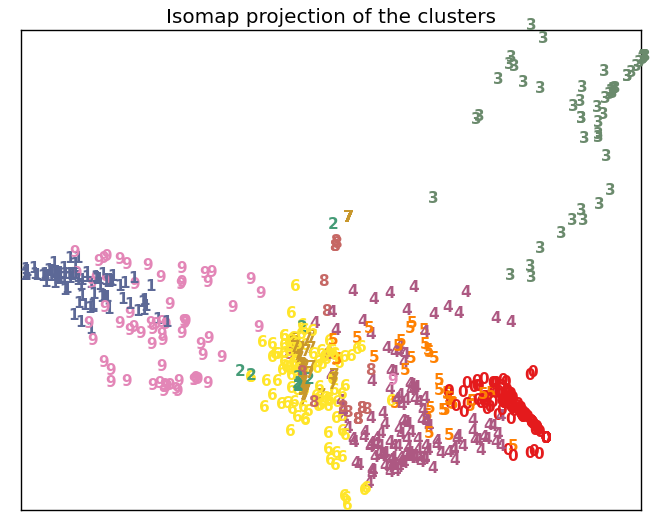
\includegraphics[width=0.65\columnwidth]{images/GMM_ISO_Z2.png}}
\caption{2 dimensional Isomap projection of a small dataset of battles for Zerg (vs Protoss) with most probable Gaussian mixture components as labels. The clusters are (Gaussian components) are labeled in colored numbers and projected in this 2 dimensional space.}
\label{fig:isoz}
\end{figure}

Figure~\ref{fig:isoz} shows a 2D Isomap \citep{isomap} projection of the battles on a small ZvP dataset. Isomap finds a low-dimensional non-linear embedding of the high dimensionality ($N$ or $N'$ dimensions, as much as unit types, the length of $U$ or $EU$) space in which we represent armies. The fact that the embedding is quasi-isometric allows us to compare the intra- and inter- clusters similarities. Most clusters seem to make sense as strong, discriminating components. The clusters identified by the numbers $2$ and $7$ (in this projection) are not so discriminative, so they probably correspond to a classic backbone that we find in several mixtures.

Figure~\ref{fig:parallelplot} shows a parallel plot of \textit{army compositions}. We removed the less frequent unit types to keep only the 8 most important unit types of the PvP match-up, and we display a 8 dimensional representation of the army composition, each vertical axis represents one dimension. Each line (trajectory in this 8 dimensional space) represents an army composition (engaged in a battle) and gives the percentage\footnote{scales are between 0 and a maximum value $\leq 100\%$, different across unit types} of each of the unit types. These lines (armies) are colored with their most probable mixture component, which are shown in the rightmost axis. We have 8 clusters (Gaussian mixtures components): this is not related to the 8 unit types used as the number of mixtures was chosen by \glos{BIC} score. Expert StarCraft players will directly recognize the clusters of typical armies, here are some of them:
\begin{itemize}
    \item Light blue corresponds to the ``Reaver Drop'' tactical squads, which aims are to transport (with the flying Shuttle) the slow Reaver (zone damage artillery) inside the opponent's base to cause massive economical damages.
    \item Red corresponds to the ``Nony'' typical army that is played in PvP (lots of Dragoons, supported by Reaver and Shuttle).
    \item Green corresponds to a High Templar and Archon-heavy army: the gas invested in such high tech units makes it that there are less Dragoons, completed by more Zealots (which cost no gas).
    \item Purple corresponds to Dark Templar (``sneaky'', as Dark Templars are invisible) special tactics (and opening).
\end{itemize}

%Each vertical (and parallel) axis represents one dimension and is scaled between $value\_min$ and $value\_max$ for the associated feature. We removed the less frequent components to keep only the 8 most important unit types of the PvP match-up. The rightmost axis corresponds to the 8 mixtures of the GMM associated to PvP army types. We colored each army (each trajectory in this 8 dimensional space) by the dominant (most probable) mixture. Expert StarCraft player will directly recognize the clusters.

\begin{figure}[h]
\centerline{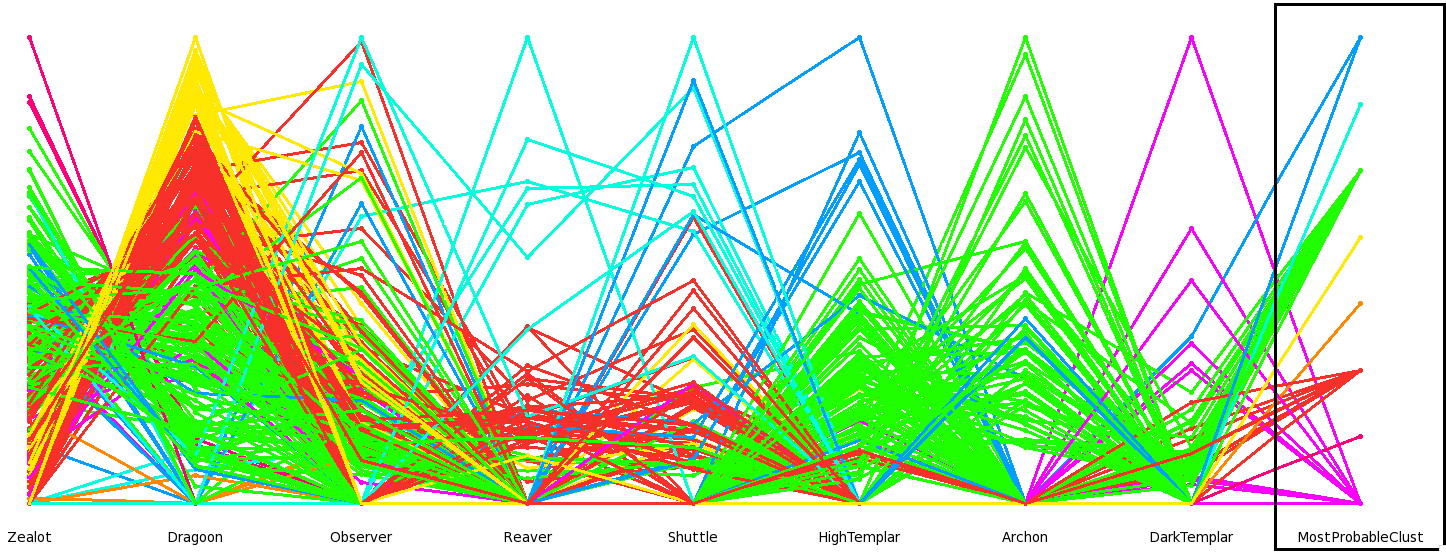
\includegraphics[width=1.12\columnwidth]{images/PvP_small.png}}
%\centerline{\includegraphics[width=2.1\columnwidth]{PvZ2.png}}
\caption{Parallel plot of a small dataset of Protoss (vs Protoss, i.e. in the PvP match-up) army clusters on most important unit types (for the match-up). Each normalized vertical axis represents the percentage of the units of the given unit type in the army composition (we didn't remove outliers, so most top (tip) vertices represent 100\%), except for the rightmost (framed) which links to the most probable GMM component. Note that several traces can (and do) go through the same edge.}
\label{fig:parallelplot}
\end{figure}

\subsubsection{Analysis of dynamics}

Figure~\ref{ecknowingecnext} showcases the dynamics of clusters components: $\PP(EC^t|EC^{t+1}$, for Zerg (vs Protoss) for $\Delta t$ of 2 minutes. The diagonal components correspond to those which do not change between $t$ and $t+1$ ($\Leftrightarrow t+2$minutes), and so it is normal that they are very high. The other components show the shift between clusters. For instance, the first line seventh column (in (0,6)) square shows a brutal transition from the first component (0) to the seventh (6). This may be the production of Mutalisks\footnote{Mutalisks are flying units which require to unlock several technologies and thus for which player save up for the production while opening their tech tree.} from a previously very low-tech army (Zerglings).
%As shown in Figure~\ref{bbq_dataflow}, this model is part of the strategy module of our next AIIDE competition bot.
%Finally, in the absence of ground truth to directly evaluate the whole model, we can only 

\begin{figure}[h]
\centerline{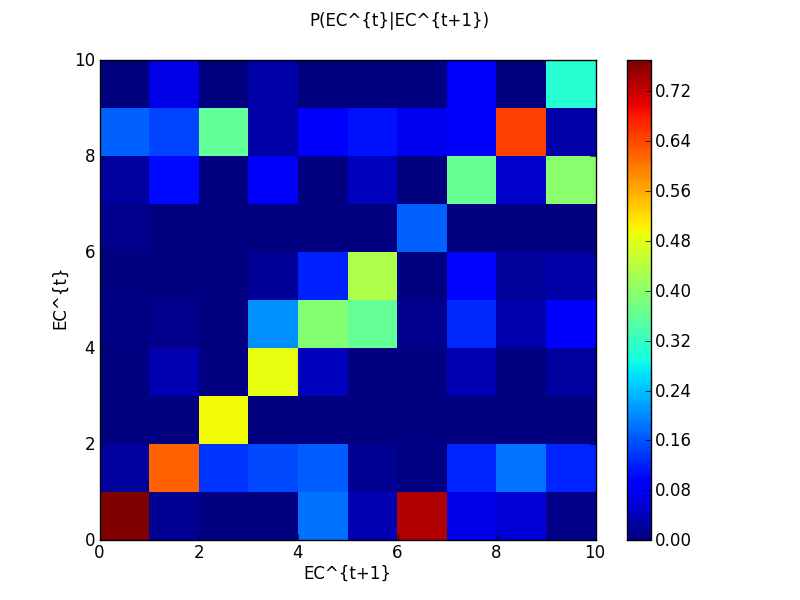
\includegraphics[width=0.76\columnwidth]{images/Z_EC_knowing_ECnext.png}}
\caption{Dynamics of clusters: $\PP(EC^t|EC^{t+1})$ for Zerg, with $\Delta t = 2$ minutes}
\label{ecknowingecnext}
\end{figure}

%\subsection{Learned Tables}

%%% \begin{figure}[htp]
%%% \centerline{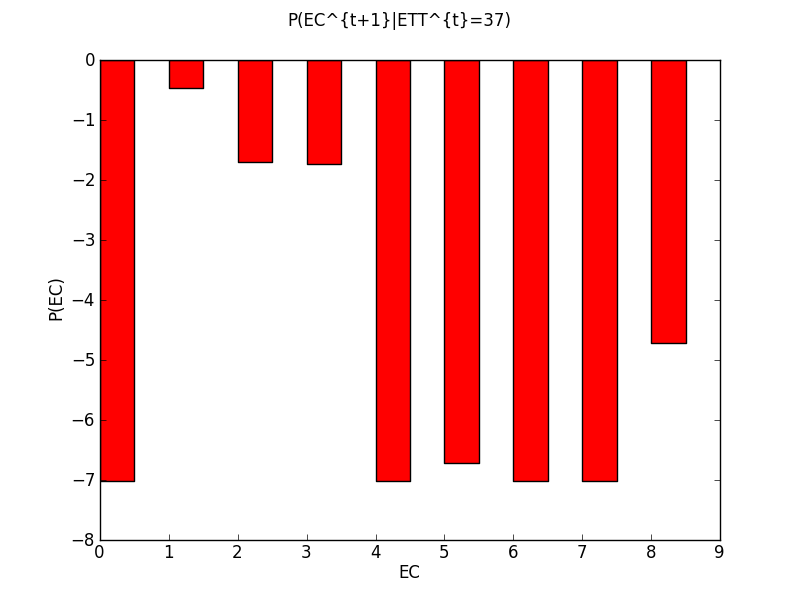
\includegraphics[width=0.92\columnwidth]{images/P_ECnext_knowing_ETT_37.png}}
%%% \caption{log $\PP(EC^{t+1}|ETT=37)$ for Protoss}
%%% \label{ecnextknowingett}
%%% \end{figure}

\subsubsection{Extensions}
\label{sec:armycompoextensions}

Here, we focused on asking $\PP(U^{t+1}|eu^t, tt^t, \lambda=1)$, and evaluated (in the absence of ground truth for full armies compositions) the two key components that are $\PP(U|C)$ (or $\PP(EU|EC)$) and $\PP(C_c|EC)$. Many other questions can be asked: $\PP(TT^t|eu^t)$ can help us adapt our tech tree development to the opponent's army. If we know the opponent's army composition only partially, we can benefit of knowledge about $ETT$ to know what is possible, but also probable, by asking $\PP(EC^t|Observations)$.
% TODO

%%% \begin{quotation}\textit{
%%% However beautiful the strategy, you should occasionally look at the results.
%%% } Winston Churchill\end{quotation}

\clearpage


\section{Conclusion}

We contributed a probabilistic model to be able to compute the distribution over openings (strategies) of the opponent in a RTS game from partial and noisy observations. %The authors are not aware of any previous works able to deal effectively with partial and noisy observations. 
The bot can adapt to the opponent's strategy as it predicts the opening with $63-68\%$ of recognition rate at 5 minutes and $>70\%$ of recognition rate at 10 minutes (up to $94\%$), while having strong robustness to noise ($>50\%$ recognition rate with $50\%$ missing observations). It can be used in production due to its low CPU (and memory) footprint. 

We also contributed a semi-supervised method to label RTS game logs (replays) with openings (strategies). Both our implementations are free software and can be found online\footnote{\url{https://github.com/SnippyHolloW/OpeningTech/}}. We use this model in our StarCraft AI competition entry bot as it enables it to deal with the incomplete knowledge gathered from scouting.

We presented a probabilistic model inferring the best army composition given what was previously seen (from replays, or previous games), integrating adaptation to the opponent with other constraints (tactics). One of the main advantages of this approach is to be able to deal natively with incomplete information, due to player's intentions, and to the fog of war in RTS. The army composition dimensionality reduction (clustering) can be applied to any game and coupled with other techniques, for instance for situation assessment in case-based planning. The results in battle outcome prediction (from few information) shows its situation assessment potential. %Finally, we will use this model in our StarCraft AI competition entry bot as it facilitates adaptive decision-making on the production plan. The main research direction is now to find a way to evaluate the full model integrated to a bot, both for performance of the bot and for the fun of a human player.

%%% Not easy to use in bot TODO
